%%
%% $Id$
%%
%% Copyright 1989-2014 MINES ParisTech
%%
%% This file is part of PIPS.
%%
%% PIPS is free software: you can redistribute it and/or modify it
%% under the terms of the GNU General Public License as published by
%% the Free Software Foundation, either version 3 of the License, or
%% any later version.
%%
%% PIPS is distributed in the hope that it will be useful, but WITHOUT ANY
%% WARRANTY; without even the implied warranty of MERCHANTABILITY or
%% FITNESS FOR A PARTICULAR PURPOSE.
%%
%% See the GNU General Public License for more details.
%%
%% You should have received a copy of the GNU General Public License
%% along with PIPS.  If not, see <http://www.gnu.org/licenses/>.
%%

% PIPS development environment documentation;
% translated and updated from dret146.f.tex

\documentclass[a4paper]{article}
\usepackage[latin9]{inputenc}
\usepackage[backref,pagebackref]{hyperref}
\makeatletter

% Test for a TeX4ht command:
\@ifundefined{HCode}{%
  % We are generating PDF, so allow to break down URL which is nicer
  % instead of ugly line overflows:
  \usepackage{breakurl}}{%
  % else we are generating HTML with TeX4ht, use plain url:
  \usepackage{url}}

\usepackage{xspace,makeidx}
\usepackage{wasysym}
\usepackage{graphicx}


%% For nice rendering of source codes:
\usepackage[hyper,procnames]{listings}
\lstset{extendedchars=true, language=C, basicstyle=\footnotesize\ttfamily, numbers=left,
  numberstyle=\tiny, stepnumber=2, numberfirstline=true, showspaces=true,
  showstringspaces=false, showtabs=true,
  tabsize=8, tab=\rightarrowfill, keywordstyle=\bf,
  stringstyle=\rmfamily, commentstyle=\rmfamily\itshape,
  index=[1][keywords],indexprocnames=true}

\sloppy

\newcommand{\LINK}[1]{\url{#1}\xspace}

\newcommand{\PipsOldWWW}{\LINK{http://www.cri.ensmp.fr/pips/}\xspace}
\newcommand{\PipsNewWWW}{\LINK{http://pips4u.org}\xspace}
\newcommand{\PipsDevGuidePDF}{\LINK{http://www.cri.ensmp.fr/pips/developer_guide.htdoc/developer_guide.pdf}}
\newcommand{\PipsDevGuideHTDOC}{\LINK{http://www.cri.ensmp.fr/pips/developer_guide.htdoc}}
\newcommand{\PipsAutotoolsGuidePDF}{\LINK{http://www.cri.ensmp.fr/pips/auto_pips.htdoc/auto_pips.pdf}}
\newcommand{\PipsAutotoolsGuideHTDOC}{\LINK{http://www.cri.ensmp.fr/pips/auto_pips.htdoc}}
\newcommand{\DoxygenSources}{\LINK{http://doxygen.pips.enstb.org/PIPS/graph}}

\title{{\Huge PIPS} \\ ~ \\ Developer Guide}

\author{
\begin{tabular}{rl}
  Corinne & \textsc{Ancourt}\\
  Fabien & \textsc{Coelho}\\
  B�atrice & \textsc{Creusillet}\\
  Serge & \textsc{Guelton}\\
  Fran�ois & \textsc{Irigoin}\\
  Pierre & \textsc{Jouvelot}\\
  Ronan & \textsc{Keryell}\\
  Arnauld & \textsc{Leservot}\\
  Alexis & \textsc{Platonoff}\\
  R�mi & \textsc{Triolet}
\end{tabular}\\
  \emph{... and so many other contributors...}
}

\date{August 1996 -- \today}

\renewcommand{\indexname}{Index}
\makeindex

% Number everything in the TOC:
\setcounter{secnumdepth}{10}
\setcounter{tocdepth}{10}

\begin{document}
\maketitle

%% show document revision:
{\small\vfill\hfill
 \verb$Id$
}

You can get a printable version of this document on\\
\PipsDevGuidePDF and a HTML version on \PipsDevGuideHTDOC. Warning if you
use the HTML version and do some copy/paste, it has been noticed that some
characters are changed, such as the \verb|'| that should be a simple plain
quote but is changed in something else that looks like a normal quote but
is not a normal quote...

The PIPS WWW site is at \PipsNewWWW.

\clearpage
\tableofcontents

\newpage

\section{Introduction}

This document aims at presenting PIPS development environment. It is
not linearly organized: PIPS is made of several, sometimes
interdependent, components.  This paper thus begins with a
presentation of PIPS directories.  Then the shell environment is
described. The next two chapters are devoted to two external tools on
which PIPS relies: NewGen and the Linear library.
Section~\ref{sec:makefiles} will then present PIPS make file policy.
Sections~\ref{sec:library_internal_organization}
and~\ref{sec:pass_organization} are devoted to PIPS libraries and
passes. The next section briefly describes some conventions usually
respected when developing in PIPS. The last two sections describe
the \emph{bug policy} of PIPS and some save and restore information.

This manual is not exhaustive. You can add your own sections and update
existing ones if you find missing or erroneous information.

The reader is supposed to be a PIPS user~\cite{Pips:96a}, and to have read
the reports about NewGen~\cite{Jouv:89,Jouv:90}. A good understanding of
\texttt{pipsmake} mechanisms would also be helpful.

\section{Getting PIPS sources}

The sources of NewGen, Linear and Pips are managed under subversion
(svn). They are accessible from anywhere in the world by the http
protocol at \url{http://scm.cri.ensmp.fr/pips.html}

\subsection{Directories overview}
\label{sec:directories-overview}

There are 5 repositories for the various files:
\begin{description}
\item[nlpmake] common makefiles for Newgen, Linear and Pips.
\item[newgen] Newgen software.
\item[linear] Linear/C3 mathematical libraries.
\item[pips] PIPS software.
\item[validation] Pips non-regression tests
\end{description}
There is also \emph{private} validation directory on another server.

The subversion repositories are organised in standard subdirectories as
advised for best subversion practices:
\begin{description}
\item[trunk] production version, should be stable enough
  to pass the validation;
\item[branches] development branches of all or part of
  the software for each developer. Developments are to be performed
  here and installed (joined, merged) once finished into \texttt{trunk};
\item[tags] tagged revisions. Note these tags are not related with the
  tags described in section~\ref{sec:using-tags}.
\end{description}

Moreover the \texttt{pips} repository includes
\begin{description}
\item[bundles:] group of softwares;
\item[bundles/trunks:] convenient extraction at once of all the 3
  softwares trunk versions ready for compilation.
\end{description}

\subsection{Building PIPS}
\label{sec:building-pips}


A crude script \texttt{setup\_pips.sh} on the web site 
(\url{http://scm.cri.ensmp.fr/svn/nlpmake/trunk/makes/setup_pips.sh})
and in \texttt{pips/trunk/makes} allows to download \texttt{polylib},
\texttt{newgen}, \texttt{linear} and \texttt{pips} and to build a local
installation of the softwares.  For instance developer \texttt{calvin} can
do the following to setup its own PIPS environment:
\begin{verbatim}
sh> setup_pips.sh /home/temp/MYPIPS calvin
...
sh> source /home/temp/MYPIPS/pipsrc.sh
sh> # enjoy
\end{verbatim}

Before you {\em enjoy} PIPS, do not worry about the many error
messages that are displayed: the header files are being recomputed
from the C files. After a while, C files should be compiled without
errors.

In order to rebuild only the PIPS infrastructure, just type
\texttt{make} into the \verb|$PIPS_ROOT| directory. If something
has gone wrong, for instance because a software component is missing
or outdated, it is advised to restart from scratch by runing
\texttt{make unbuild} before trying again.

For more information about the PIPS Makefile infrastructure, see
Section~\ref{sec:underst-makef-infr}.

\subsection{Important note}

It is important to realize that:
\begin{enumerate}
\item PIPS build is much more efficiently if it is stored on local disks rather
  than on remote directories accessed through the network (\emph{e.g.} via NFS).
  Hence the \texttt{/home/temp} directory choice in the above axample.
\item the local copy editions are not saved unless commits are performed.
\item in a standard development, commits should not be made directly under
  the \texttt{trunk}, but rather in development branches, see the next section.
\item on some Unises, the \texttt{/tmp} temporary directories may be cleaned
  on reboots, which can be triggered by power failures. So you could try
  \texttt{/var/tmp} that is usually not cleaned-up during the boot phase.
\end{enumerate}


\section{Developing environment}
\label{sec:devel-envir}


\subsection{Browsing and documenting the source files with Doxygen}
\label{sec:brows-source-files}

To help digging into the sources, Doxygen is used to generate an
interactive on-line version of the sources that can be seen at
\DoxygenSources. The call and caller graphs are useful to figure out what
are the functions used, and more subtly what are the functions that call a
given function (if you need to verify a function is correctly used or you
want to change a function name).

As an experimented user, you may need to generate them again. The
\texttt{doxygen} \emph{make} target is propagated downwards down to the
various \texttt{doxygen} directories in the products (NewGen, Linear and
PIPS).

To push them on the WWW, you can use a \texttt{make doxygen-publish}, if
you have the right access.

The \texttt{make} target \texttt{doxygen-plain}
or \texttt{doxygen-graph} can be used to generate only a documentation
without or with call and caller graphs. Note that generating the graph
version for PIPS lasts several hours on a 2009 computer...

Of course, developers in PIPS should use the Doxygen syntax to have a more
useful documentation.

Modules and submodules in Doxygen are quite useful to group related
objects and structure concepts in the documentation. For an example, have
a look to \verb|@defgroup|, \verb|@addtogroup|, \verb|@{| and \verb|@}| in
\verb|newgen/src/genC/genClib.c| and the resulting module \emph{NewGen
  quick and intelligent recursion on objects (visitor pattern)} and its
submodules in the documentation. Be careful: a title group must be on the
same line and cannot be split !

A good practice should be to present main useful functions and concepts to
know by a PIPS programmer as modules and submodules.

\subsection{Developing with Eclipse}
\label{sec:developing-with-eclipse}

Eclipse is a multi-language software development environment comprising an 
integrated development environment (IDE) and an extensible plug-in system. 

You have to use an eclipse installation with CDT plugin
(have a look at \url{http://www.eclipse.org/cdt}) to be able to use eclipse for C/C++
development.


\subsubsection{Workspace/Project creation}

In Eclipse you have workspace and project concept. The latter is like a
repository, or a subtree of a source location. In PIPS it can be a pass, whole
pips or linear or newgen, or all of them in one shot !

A workspace is a set of projects that are usually related, loaded in memory, and
indexed while working. For instance if you want Eclipse to provide some 
navigation features in newgen source code while working on PIPS project, you 
need to have both project in the same workspace.

The creation of a project in a workspace is easy and suppose that you already 
have PIPS sources somewhere on you hard drive.

\begin{center}
\noindent
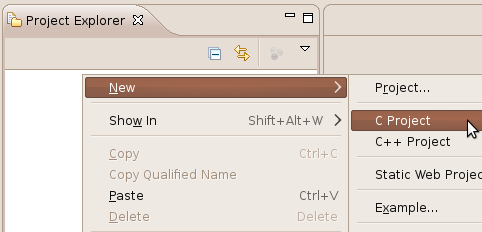
\includegraphics[scale=0.4]{eclipse/eclipse-project-creation-1.png}
\end{center}
\begin{center}
\noindent
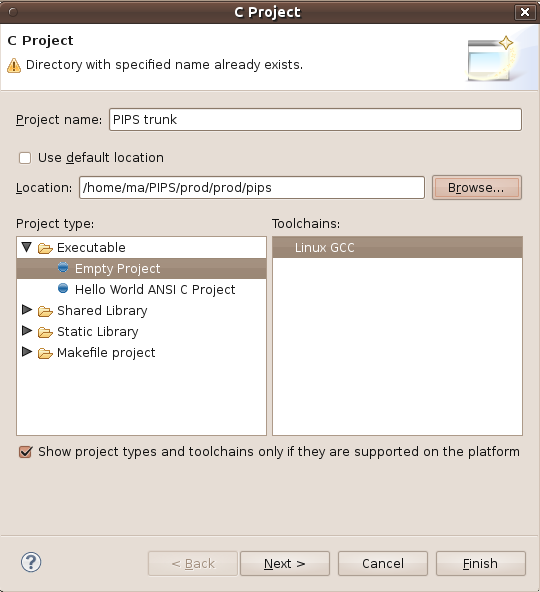
\includegraphics[scale=0.35]{eclipse/eclipse-project-creation-2.png}
\end{center}

First use menu \textit{File} $=>$ \textit{New} $=>$ \textit{Project} or 
right-click and contextual menu as shown on 
the screenshot, then give a project name, uncheck the checkbox to enable browsing
an existing location, and find your PIPS source directory. Click finish and you
have now a fresh new PIPS project in Eclipse. It may overload your computer for 
a little while indexing the whole project, you can see the progression in the
status bar down the Eclipse window. Index can be rebuild at any time using 
right click on project root.

You should really repeat this operation for Newgen and Linear project.

\subsubsection{Missing includes}

Try to open some source files, for instance src/Libs/chains/chains.c and scroll
a little. You'll find some part of the underlined by Eclipse. Eclipse just like
your favorite compiler detect undefined symbol and report it to you in a 
friendly way.

\begin{center}
\noindent
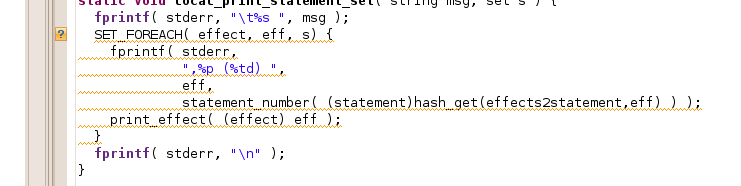
\includegraphics[scale=0.4]{eclipse/eclipse-missing-includes.png}
\end{center}

We are missing Newgen and Linear includes, we have only default Eclipse includes :

\begin{center}
\noindent
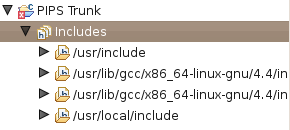
\includegraphics[scale=0.4]{eclipse/eclipse-missing-includes-2.png}
\end{center}

Select project root and push \textit{alt+enter} or right click on it and
select properties item in the contextual menu. Then go to C/C++ General
submenu and select Paths and Symbols. In the Includes tab select language
GNU C in the left part and click add. Then choose \textit{Workspace...}
and find you \texttt{pips/include/} dir. Repeat the same operation for
including Newgen and Linear include dirs.

\begin{center}
\noindent
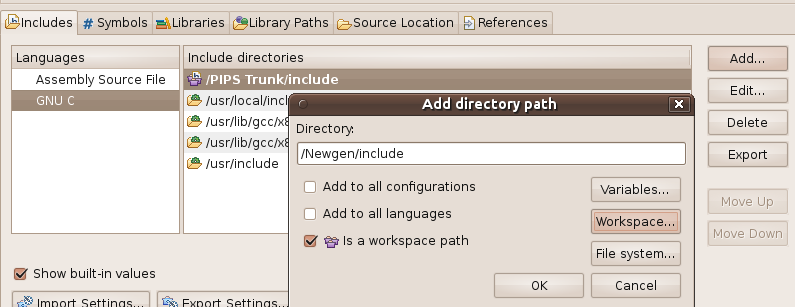
\includegraphics[scale=0.35]{eclipse/eclipse-project-creation-add-includes.png}
\end{center}

Validate two times and accept to rebuild the index when Eclipse ask. After index
rebuilding you can observe that the code is no longer underlined. :-)

\subsubsection{Benefits from Eclipse power}

Eclipse provide many features to help you becoming more productive. Firstly is
the vertical bar just right to the code :

\begin{center}
\noindent
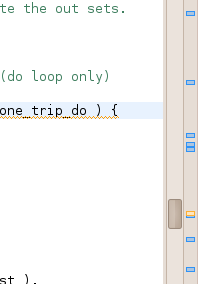
\includegraphics[scale=0.4]{eclipse/eclipse-shortcut-vertical-bar.png}
\end{center}

Clicking on this bar make you move inside a source file quickly, there is kind
of colored \textit{post it} that are shortcut. Color informs you from what's
going on at this point of the source. For instance red is an error, white is 
occurence of currently focused variable (very useful !), and blue are occurence
of \textit{FIXME} stickers in comments (use it !). Yes I know that there's a lot 
of blue post it in chains ;-)

\begin{center}
\noindent
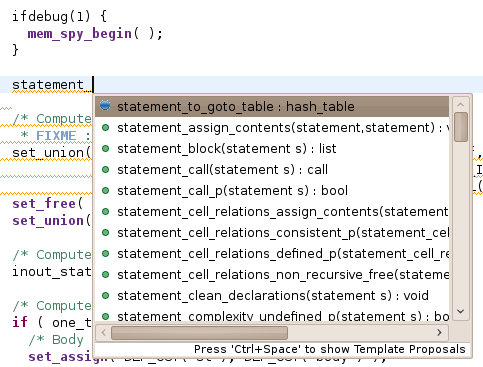
\includegraphics[scale=0.4]{eclipse/eclipse-completion.png}
\end{center}

Eclipse provide you some completion capabilities, try to write the begin of a 
symbol at some place in the code and hit \textit{ctrl+enter}

You can easily find the definition of a symbol, even if it's located in another 
source file or even another project. The magic key is F3, try it on 
\textit{set\_make} for instance, the first press will bring you to the header
in Newgen/include and the second press will bring you to the definition of the 
function. You can always go back using \textit{alt+left arrow}

Another very pleasant feature is the lookup windows, which you can get using 
\textit{ctrl+alt+t} or menu \textit{Navigate} $=>$ \textit{Open element}. You 
can use the star as a joker for searching symbol by their name.

\begin{center}
\noindent
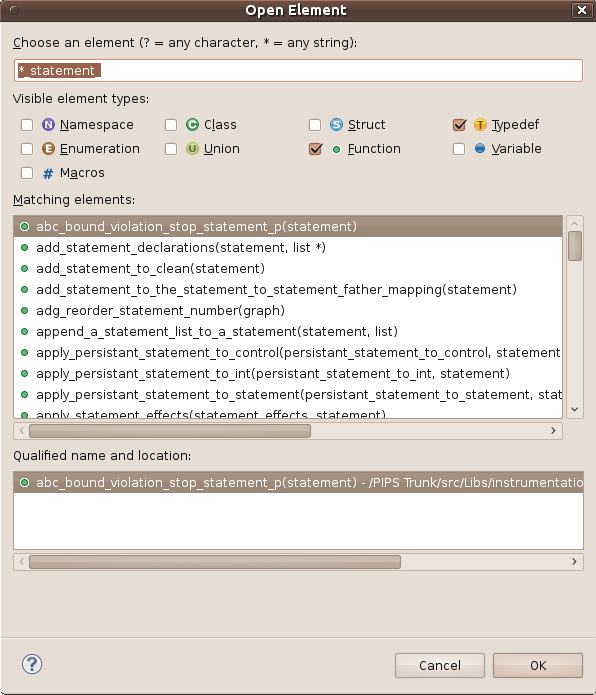
\includegraphics[scale=0.35]{eclipse/eclipse-symbol-lookup.png}
\end{center}

PIPS/Newgen make high usage of macro, Eclipse has a powerful macro expansion 
step-by-step. You can have a quick view by moving your pointer over the macro. 
Or you can interactively develop the macro with a right click on it and 
\textit{Explore Macro Expansion} or pressing \textit{ctrl+=} after having 
selected it.

\textit{ctrl+shift+g} is one of my favorite feature :-). Used on a function it'll
show you every call site in the workspace !

Others entries in the menu \textit{Navigate} provide also intersting features, 
try them !

Eclipse provide also some refactoring power, use the right click or the menu and
select \textit{Rename...}. You can rename a variable so as a function ! Every 
usage and declaration in the workspace will be updated. Obviously, it'll be 
longer for a widely used newgen function than for a static function !



\subsubsection{Using team working plugin, aka. SVN/GIT for Eclipse}

TODO

\subsubsection{Building from Eclipse}

TODO


\subsection{Developing with the Emacs editor}
\label{sec:developing-with-emacs}

There are many modes in Emacs that can help developments in PIPS.

To compile the sources you can use the menu \texttt{Tools/Compile...}. It
presents errors in red and if you click on them you jump to the sources at
the right location.

The check-compilation-errors-on-the-fly is quite fun (it is equivalent in
programming to the on-the-fly spell checker \texttt{flyspell-mode}). PIPS
makefiles support it. Try it with \texttt{M-x flymake-mode}.

The \texttt{speedbar} mode helps with a navigation window. More descrete,
to have access from the menu to functions and other symbols in the local
source file, test the \texttt{imenu-add-to-menubar} Emacs function.

You can use tags to index source files as explained in
section~\ref{sec:using-tags}.

Most PIPS contributors use Emacs to develop in PIPS, so some goodies have
been added to ease those developers.

Have a look for example at section~\ref{sec:newgen} for debugging. You
should use the \texttt{gud-tooltip-modes} to display the value of an
object under the mouse. Setting the \texttt{gdb-many-windows} to
\texttt{t} transform Emacs (from version 22) in an interesting graphical
IDE. You can select a frame by just clicking it and so on.

Most documentation (like the one you are reading) is written in LaTeX and
some parts even use literate programming with a \LaTeX{} base, so the
AUCTeX, PreviewLaTeX and RefTeX mode are quite useful.


\subsection{Using tags to index source files and to ease access in your
  text editor}
\label{sec:using-tags}

Many macros and functions are available from the Linear and NewGen
libraries, but also in PIPS. Their source code can be retrieved using the
\emph{tags} indexing mechanism under editors such as \textbf{emacs} or
\textbf{vi}. You should notice that this notion of tags is unrelated to
the tags in a version control systems as exposed in
\S~\ref{sec:full-branch}.

So the PIPS makefiles can generate tags index files to find the definition
of symbols in the source files with your favorite editor and it is highly
recommended to use the Emacs or VI editors to benefit from the tags.  For
example in Emacs, you can find, by typing a \texttt{M-.} on an identifier,
the location where it is defined, \texttt{M-,} allows to find another
location. Note that completion with \texttt{TAB} works with tag searching
too. With \textbf{vi}, you can use \texttt{C-]} to jump on a definition of
an identifier.


PIPS can produce tags files for VI by invoking \verb|make CTAGS| or tags
for Emacs by invoking \verb|make TAGS| in the PIPS \texttt{prod} top
directory and it will produce the tags files into the \texttt{linear},
\texttt{newgen} and \texttt{pips} subdirectories.

To build the tags for both VI and Emacs, just use a simple \texttt{make
  tags}.  The tags files at the PIPS top directories need to be remade
regularly to have an up to date version of the index.  should be used for
\textbf{vi} users.

You can also build specifically the tags for a development version of PIPS
for example by making these tags explicitly in the \texttt{newgen/trunk},
\texttt{pips/trunk} and \texttt{linear/trunk} directories.

Then you need to configure your editor to use these tags files, for
example in Emacs by using the customization of the \texttt{Tags Table
  List} with the \texttt{Options/Customize Emacs} menu or more
directly in you \texttt{.emacs} with stuff like:
\begin{itemize}
\item for a production version of the tags :
\begin{verbatim}
(custom-set-variables
  ;; ...
 '(tags-table-list (quote
    ("/home/keryell/projets/PIPS/MYPIPS/prod/newgen/TAGS"
     "/home/keryell/projets/PIPS/MYPIPS/prod/linear/TAGS"
     "/home/keryell/projets/PIPS/MYPIPS/prod/pips/TAGS")))
 )
\end{verbatim}
\item for a development version of the tags :
\begin{verbatim}
(custom-set-variables
  ;; ...
 '(tags-table-list (quote
    ("/home/keryell/projets/PIPS/svn/newgen/trunk/TAGS"
     "/home/keryell/projets/PIPS/svn/linear/trunk/TAGS"
     "/home/keryell/projets/PIPS/svn/pips/trunk/TAGS")))
 )
\end{verbatim}
\end{itemize}

\subsection{Using cscope to navigate source file}

In a way similar to \texttt{ctags}, \texttt{make cscope}
\footnote{\texttt{make cscope.out} for nlpmake users} creates a database
suitable for use with the \texttt{cscope} tool.
This tool make it possible to find callers, definition or declaration of a function,
enabling advanced code navigation not possible with tags.

Here are the relevant lines for a \texttt{vim} configuration, to be added to
\texttt{.vim/ftplugin/c.vim}
\begin{lstlisting}
" cscope
if has("cscope")
	set csto=0
	set cst
	set nocsverb
	" add any database in current directory
	if filereadable("cscope.out")
		cs add cscope.out
		" else add database pointed to by environment
	elseif $CSCOPE_DB != ""
		cs add $CSCOPE_DB
	endif
	set csverb
endif
\end{lstlisting}



\subsection{Developing PIPS under SVN}
\label{sec:dev-svn}

A basic understanding of subversion operations and concepts such as
\emph{repository, checkout, status, commit} are necessary to develop in
PIPS.  See for instance the SVN book at
\LINK{http://svnbook.red-bean.com/} and other resources on the
Internet. This section assumes that you have a recent version of svn,
version \textbf{1.5} or above, as these versions greatly improve the
management of branches.

The development policy within the PIPS-related software is that the
\texttt{trunk} version should hold a production quality software which
should pass all non-regression tests that run daily at CRI and elsewhere.
Thus day-to-day development should not occur within this part, but in
independent per-developer \texttt{branches} which should be validated
before being merged back into the \texttt{trunk}.

SVN can manage properties about files which help portability by
declaring the end-of-line policy, the mime-type and so on.
We recommand that you add the following to your
\texttt{.subversion/config} file:
{\scriptsize
\begin{verbatim}
# in section [miscellany]
enable-auto-props = yes

[auto-props]
# pips-related props
*.f = svn:eol-style=native;svn:keywords=Id URL;svn:mime-type=text/x-fortran
*.F = svn:eol-style=native;svn:keywords=Id URL;svn:mime-type=text/x-fortran
*.f77 = svn:eol-style=native;svn:keywords=Id URL;svn:mime-type=text/x-fortran
*.f90 = svn:eol-style=native;svn:keywords=Id URL;svn:mime-type=text/x-fortran
*.c = svn:eol-style=native;svn:keywords=Id URL;svn:mime-type=text/x-c
*.h = svn:eol-style=native;svn:keywords=Id URL;svn:mime-type=text/x-c
*.sh = svn:eol-style=native;svn:executable;svn:keywords=Id URL;svn:mime-type=text/x-sh
*.pl = svn:eol-style=native;svn:executable;svn:keywords=Id URL;svn:mime-type=text/x-script.perl
Makefile = svn:eol-style=native;svn:keywords=Id URL;svn:mime-type=text/x-make
*.mk = svn:eol-style=native;svn:keywords=Id URL;svn:mime-type=text/x-make
*.tex = svn:eol-style=native;svn:keywords=Id URL;svn:mime-type=text/x-tex
*.bib = svn:eol-style=native;svn:keywords=Id URL;svn:mime-type=text/x-bibtex
*.txt = svn:eol-style=native;svn:keywords=Id URL;svn:mime-type=text/plain
*.py = svn:eol-style=native;svn:keywords=Id;svn:mime-type=text/x-python
*.tpips = svn:eol-style=native;svn:mime-type=text/x-tpips
# and other property settings that you could find useful
*.png = svn:mime-type=image/png
*.jpg = svn:mime-type=image/jpeg
*.csv = svn:eol-style=native;svn:mime-type=text/csv
*.sql = svn:eol-style=native;svn:keywords=Id URL;svn:mime-type=text/x-sql
\end{verbatim}
}


\subsubsection{PIPS development branches}
\label{sec:pips-devel-branch}

If you are doing something non trivial or do not have commit rights on
pips' trunk, you shoud develop in a branch of your own. To do so:

\begin{enumerate}
\item Obtain an svn user account on \texttt{scm.cri.ensmp.fr}
  by asking for it to Fabien Coelho.

  For instance, a login \texttt{calvin} and some password may be attributed.
  Calvin will have his own development area under \texttt{branches/calvin}
  in the subversion repository.

  The developer branch is private by default. It means that what you
  do in the branch is your own business, and no message is sent to the
  world on commits. For interns, the default policy is to send a
  message to the intern and the developer(s) responsible for his/her
  work.

  For HPC-Project related accounts, branch commits are send to the
  corresponding list.

  \textbf{Please do commit your work at least once a day, even if it does not
  work yet!}

\item Extract your own PIPS with the setup script (\texttt{setup\_pips.sh})
  mentionned above.
  The resulting directory may contain at the end of the building process:
  \begin{description}
  \item[prod] compiled production version of \texttt{pips},
    \texttt{newgen}, \texttt{linear} and the external \texttt{polylib}
    library;

    %% should the dev directory be called calvin?
    %% however how to differentiate newgen/linear/pips branches in such cases?
  \item[pips\_dev] Calvin's private development area which points to
    \texttt{branches/calvin} and should be empty at the beginning;
    It can be created afterwards with a manual checkout if necessary in
    your \texttt{MYPIPS} directory (or wherever you want) later with:
{\small
\begin{verbatim}
sh> svn co https://scm.cri.ensmp.fr/svn/pips/branches/calvin pips_dev
\end{verbatim}
}
    Branches may also be used for \emph{linear} and \emph{newgen} development,
    in which case the local directory name for the checkout should be called
    \texttt{linear\_dev} or \texttt{newgen\_dev} respectively.
  \item[validation] a working copy of pips non regression tests for
    validation.  See Sections~\ref{sec:devel-branch-valid} \&
    \ref{sec:validation} for informations about the validation, and then
    really read the \texttt{README} file to run it.
  \item[pipsrc.sh] sh-compatible shell initialization;
  \item[pipsrc.csh] csh-compatible shell initialization.
  \end{description}

\item Create your own development branch for all PIPS:
{\small
\begin{verbatim}
sh> cd pips_dev
sh> svn cp https://scm.cri.ensmp.fr/svn/pips/trunk my-branch-name
sh> svn commit my-branch-name
\end{verbatim}
}
  It creates a new branch as a working copy, which is then committed
  to the repository.

  The idea is to branch a whole PIPS copy since it ensures that the
  developments you do in many places in PIPS (even at some place you would
  not have expected when you created the branch!) can be committed
  atomically.

  \textbf{CAUTION!}
  take care to create branches only for the \emph{trunk}. Creating
  branches for a subdirectory breaks svn bookkeeping.

\item Develop, test, commit within your branch\ldots

  \textbf{CAUTION!}  When testing, check that the
  \verb.PIPS_ROOT. environment variable points to your development branch
  instead of the trunk.  You may also check for the right settings for
  \verb.EXTERN_ROOT. \verb.NEWGEN_ROOT. and \verb.LINEAR_ROOT. variables,
  as well as your \verb.PATH. to ensure that the right executable is
  used. Have a look to \S~\ref{sec:shell} for more information.

\item To merge into your branch on-going developments by other people from
  trunk, first you need to have already committed your branch and
  then, in your branch (and no other directory above or under):
  {\small
\begin{verbatim}
sh> cd my-branch-name
# the above cd is useful: it aims at going into the branch root,
# i.e. the copy of the "trunk", before merging.
sh> svn merge https://scm.cri.ensmp.fr/svn/pips/trunk
# this does the merging into the branch working copy
# - consider options -x -b or -x -w
#   to ignore space-related changes
# - if there are conflicts, choose 'p' (postpone)
#   and deal with them later.
sh> svn status
# check for conflicts (C state) or other issues, and resolve them.
sh> svn commit
\end{verbatim}
  }

  With \texttt{svn 1.6} it will be possible to type only:
  {\small
\begin{verbatim}
sh> cd my-branch-name
sh> svn merge ^/trunk
# consider options -x -b or -x -w
# to ignore space-related changes
sh> svn status
sh> svn commit
\end{verbatim}
  }

  If you change your initial idea, you can always revert back to your
  original version \emph{if it was committed before} with a:
  {\small
\begin{verbatim}
svn revert -R .
\end{verbatim}
  }

  Well, it does not remove the new files that may be created previously in
  your local copy by the merge procedure, it only delete their meta-data
  from the subversion point of view. So the cleaner way is to merge into a
  new working copy of the trunk so that if things go wrong you can simply
  delete the working copy.

  To know about where you are compared to the trunk, you can try a:
  {\small
\begin{verbatim}
svn diff https://scm.cri.ensmp.fr/svn/pips/branches/calvin/graph \
   https://scm.cri.ensmp.fr/svn/pips/trunk
\end{verbatim}
  }

  \textbf{CAUTION!}
  Merging must be done at the root of the branch, that is the
  directory which correspond to the \texttt{trunk}.
  \textbf{DO NOT} merge in a subdirectory as it breaks svn bookkeeping
  for subsequent merges, and will result in tree numerous conflicts, which
  when resolved may be rejected by the pre-commit hook.

\item When you are done with your developments, they are committed into
  your branch, you want to install them back to the pips trunk.
  You must have write access to the \texttt{trunk} in order to do the commit.
  First, you must bring your branch up-to-date with respect to the
  \texttt{trunk}, which is the \texttt{merge} described above.
  Then you can reintegrate your changes to the \texttt{trunk}:
{\small
\begin{verbatim}
sh> cd prod/pips  # cd in your pips trunk copy, or better a fresh copy
sh> svn mergeinfo \
  https://scm.cri.ensmp.fr/svn/pips/branches/calvin/my-branch-name \
  --show-revs eligible
# revisions that need be reintegrated...
sh> svn merge \
  https://scm.cri.ensmp.fr/svn/pips/branches/calvin/my-branch-name \
  --reintegrate
# consider options -x -b or -x -w
# to ignore space-related changes
# there should be no issue found on a reintegration.
sh> svn status
# the status or diff should reflect the branch changes.
# the ' M .' reflects the changes of branch bookkeeping informations.
# DO NOT EDIT ANY OF THE FILE
# DO NOT COMMIT FILES SEPARATELY
# you may need to do additional "svn up" if there are external
# commits between the merge & its commit.
sh> svn commit

# It's mandatory to remove the branch after it has been reintregrated !!
sh> cd where_the_branch_is
sh> svn rm my-branch-name
sh> svn commit my-branch-name
\end{verbatim}
}

  \textbf{CAUTION!} it is important to merge and commit at the
  \texttt{trunk} level, all in one go.
  If the merging or commit is done on a subdirectory, it breaks svn
  merge bookkeeping used my the automatic mergings and reintegration
  because \texttt{svn:mergeinfo} properties are added on these
  subdirectories: when set, they must be manually removed in order to fix.

\item When your are fully done with your branch, you may remove it.
  {\small
\begin{verbatim}
sh> cd pips_dev
sh> svn remove my-branch-name
sh> svn commit
\end{verbatim}
  }
\end{enumerate}


\subsubsection{Developing in a branch? Validate before merging!}
\label{sec:devel-branch-valid}

Do not forget that if you or someone else merges your branch into the
trunk, things must be compiled with an up-to-date copy of all the PIPS
environment and validated first against the last global PIPS validation to
avoid havoc for the other PIPS developers.

Here is a typical behaviour you should follow:
\begin{enumerate}
\item update your production copy of PIPS and all (the \texttt{prod}) with
  \texttt{svn up}, recompile the production version and apply the
  validation against it to have a reference;
\item do/correct your development;\label{item:do_correct}
\item compile and validate\footnote{If you work in a localized part of
    PIPS, it may be interesting to first run a reduced validation, such as
    if you work in the C parser, it is obvious that at least the C parser
    should work so you can run, instead a full validation, only a
    \texttt{make TARGET=C\_syntax validate}. Of course, if it pass the
    validation, do not forget to run a full validation
    afterwards.};\label{item:compile_validate}
\item if it does not work, go to point \ref{item:do_correct}
\item merge the \texttt{trunk} into your branch to get synchronized with
  the PIPS outside world;\label{item:pull}
\item commit your branch saying you have merged the universe into your
  branch\footnote{You commit to avoid having in your working copy both
    modifications from the trunk and further eventual corrections you will
    do to have things working, which is a bad practice from a tracking
    point of view. Between 2 commit points it is better to have only one
    kind of modification so you can easily see what has changed, when and
    who is guilty...};
\item compile and validate;
\item if it does not work, go to point \ref{item:do_correct};
\item if you are happy with the validation, merge your beautiful work into
  the PIPS Holly trunk with \texttt{svn merge -\,-reintegrate}
  (\S~\ref{sec:pips-devel-branch}) so that all the PIPS community can
  congratulate you;
\item if the merge fails because someone insidiously committed her
  valuable work just since your last synchronization from the trunk, go to
  step \ref{item:pull}, else you have to delete your branch, it can't be use
  anymore after having been reintegrated !
\end{enumerate}

For more information about the validation process, have a look to
\S~\ref{sec:validation}. Since your validation mileage may vary according
to your target architecture because of bugs or limitations (little or big
Endian, native 32-bit or 64 bit architecture...) you should try to
validate on various architectures.

\subsubsection{Creating FULL branches or tags}
\label{sec:full-branch}

The \texttt{pips\_branch} script creates a full branch or tag of the
same name in all 5 repositories (makefiles, 3 softwares, validation),
and a \emph{bundle} entry to extract all these files at once.
The script needs full write permissions to all five repositories, thus
it is restricted to core developers. The help option provides help.

To create a \texttt{foo/bla} named branch from trunk try:
\begin{verbatim}
  sh> pips_branch -v -v trunk branches foo/bla
\end{verbatim}
It shows the various \texttt{svn} commands which are going to be issued.
If you are happy with them, do that again with the \texttt{-D} option
to actually run them. The created \emph{bundle} can be extracted with:
\begin{verbatim}
  sh> svn co https://scm.cri.ensmp.fr/svn/pips/bundles/foo/bla
  extracting newgen... linear... pips... validation... nlpmake...
\end{verbatim}

Note that the \texttt{-R} options allows to fix the revision number to
consider from each repository, instead of using the head revision.

\subsubsection{Understanding the Makefile infrastructure inside the SVN
  infrastructure}
\label{sec:underst-makef-infr}

This section is to be skipped at first reading and is only of interest for
people wanting to modify more globally the PIPS infrastructure.

The compilation directories are managed by some global variables
initialized as described in section~\ref{sec:shell}.

If you compile into a directory, in the \texttt{prod} directory installed by
the installation script, your branch directory or whatever, the compiled
stuff from a directory goes to the corresponding \texttt{bin lib}
directories next to the \texttt{src} directory.
%%
The \emph{Makefile} definitions are taken from the corresponding
\texttt{makes} directory next to the \texttt{src} sources.

For example, if you have a local PIPS copy in the \texttt{svn/pips/trunk}
and you compile with \texttt{make}, it will build against
\verb/$NEWGEN_ROOT/ and \verb/$LINEAR_ROOT/, it will install into
\texttt{bin} and will use \emph{Makefile} stuff from \texttt{makes}.
So if you want to modify the \emph{Makefile} infrastructure, modify
the \texttt{makes} directory and commit. It will be committed into the
\texttt{svn/nlpmake/trunk} repository anyway.

There is also another more modern build infrastructure you may use instead
of this one that is described in the companion document of this one that
describes the new \texttt{autotools} build infrastructure:
\PipsAutotoolsGuidePDF{} and \PipsAutotoolsGuideHTDOC{}


\subsection{The nomadic developer}
\label{sec:nomadic}

The SVN centralized development model assumes that you are connected to
the repository. If you are stuck in a train between Paris and Brest (in
the very far west of France \smiley), you may find it inconvenient not to
be able to access the repository history and other details about previous
commits, especially if the current version is broken.  In order to help
preventing this situation anyway, PIPS is checked every minute and
possibly fully recompiled.

So if you are Ronan, consider using \texttt{git-svn} or \texttt{svk}
to have full copy of your branch or of the trunk on your laptop. Then
you can develop offline including branching and commits. You will be
able to push back into the SVN server your changes once you get back
to civilized surroundings.

Why not switch all this stuff to \texttt{git}, which is so
\emph{cool}? There are several reasons:
\begin{description}
\item[system] we already use subversion extensively at CRI for many
  projects, which are backed-up regularly (hourly \texttt{svnsync},
  daily night on tape backup).
\item[change management] subversion is hard enough, and learning a new
  tool with a different model is a significant investment, which can
  only be justified with a clear added value.
  GIT is harder to understand and to learn than SVN.
\item[backup] with GIT, there is no natural backup on commits, as they are
  stored locally: you have to push your changes. This induces a greater
  risk of losing developments.
\item[development model] a centralized model helps with the development
  coordination, with distributing mails on commits to revelant
  recipients, and so on. It helps to access all developer branches.
\item[nomadic] the nomadic developer special needs can be addressed by
  other means (\emph{e.g.} git-svn) without necessarily impacting the
  common infrastructure.
\item[coordination] is easier in a centralized models, where source
  divergence can be detected in one place, and possibly managed.
\end{description}

At HPC Project we use GIT with central servers, so the previous points of
view from CRI are rather out-of-focus\ldots

\subsubsection{Keeping a local copy of PIPS repositories with \texttt{svnsync}}
\label{sec:svnsync}

In order to access pips logs at anytime, you may consider keeping
a local copy of pips repositories anywhere you want, including on a
laptop, with the \texttt{svnsync} command.
The operation is mostly network bound: it takes under 15~minutes
to copy the whole history of the 5~repositories from the CRI LAN.
Beware that this copy must only be used read-only.

{\scriptsize
\begin{verbatim}
mkdir PIPS_SVN
cd PIPS_SVN
# initialize the copy
for r in nlpmake newgen linear pips validation ; do
  svnadmin create $r
  echo -e '#!/bin/sh\nexit 0' > $r/hooks/pre-revprop-change
  chmod +x $r/hooks/pre-revprop-change
  svnsync init file://$PWD/$r https://scm.cri.ensmp.fr/svn/$r
done

# then sync from time to time.
# it takes a some time the first time, obviously...
# in the PIPS_SVN directory do:
for r in nlpmake newgen linear pips validation ; do
  svnsync sync file://$PWD/$r
done
\end{verbatim}
}

\subsubsection{The git-svn gateway}
\label{sec:git-svn}

This section assumes that you have a good working knowledge of both
GIT and SVN. If you use GIT, do not forget to save your repository
regularly.

\texttt{git-svn} is a porcelain which ensures a limited compatibility
between a centralized SVN repository and a local GIT repository. It
provides the ability to pull/push commits from a single branch in an
SVN repository. Beware of the limitations:
\begin{itemize}
\item branches and tags in more than one directory (we use
  subdirectories in \texttt{branches}) are not clearly managed;
\item SVN properties are mostly ignored (ignore, externals\ldots);
\item cloning the pips tree does take a long time;
\item it does not know about branch management in subversion (since 1.5),
  so merging an svn branch from git and pushing back the result breaks
  svn branch management;
\item commit messages pushed from \texttt{git-svn} may be quite unhelpful;
\end{itemize}
So just use \texttt{git-svn} to manage an already created branch which
will be seen as the \texttt{master} branch by GIT. Creating new
branches under GIT and hoping to have them appearing under SVN seems
hopeless.

Here is a summary of operations\footnote{ISTM that this ammended version does not work
or is at least error prone. Fabien.}:
{\scriptsize
\begin{verbatim}
# create copies of the repositories' trunks that
# you may wish to edit. Example:
git svn clone --stdlayout https://scm.cri.ensmp.fr/svn/nlpmake

git svn clone --stdlayout https://scm.cri.ensmp.fr/svn/newgen
ln -s ../nlpmake/makes newgen/makes
echo /makes >> newgen/.git/info/exclude

git svn clone --stdlayout https://scm.cri.ensmp.fr/svn/linear
ln -s ../nlpmake/makes linear/makes
echo /makes >> linear/.git/info/exclude

# This one takes 1 or 2 hours on a file repos...
# Deal with the fact that branches are hierarchized per user,
# so if I'm the user coelho
git svn clone --stdlayout -branches=branches/coelho \
    https://scm.cri.ensmp.fr/svn/pips
ln -s ../nlpmake/makes pips/makes
echo /makes >> pips/.git/info/exclude

git svn clone --stdlayout https://scm.cri.ensmp.fr/svn/validation

# live your life within git
# what about properties?
# svn:ignore & .git/info/exclude?

# when online, update/resync from svn
for d in newgen linear pips nlpmake validation; do
  pushd $d
  # consider running with option --dry-run
  git svn rebase
  popd
done

# push your local commits to svn
cd pips
git svn dcommit --dry-run
git svn dcommit
\end{verbatim}
}

Since in the PIPS repositories there is also some quite old history (based
on RCS and SCCS\footnote{introduced at CRI by Keryell Ronan on May 17, 1993}),
the history does not fit into classical SVN \texttt{trunk},
\texttt{branches} and \texttt{tags} and thus cannot either be understood well by \texttt{git-svn}.
%%
So for ultimate PIPS historian which does not want to use \texttt{svnsync}, you can have also a
copy of the repository with \texttt{git-svn} without using the
\texttt{trunk}/\texttt{branches}/\texttt{tags} convention.
%%
For this, just use a plain \texttt{git-svn} with:
\begin{verbatim}
git svn clone https://scm.cri.ensmp.fr/svn/nlpmake
git svn clone https://scm.cri.ensmp.fr/svn/linear
git svn clone https://scm.cri.ensmp.fr/svn/newgen
git svn clone https://scm.cri.ensmp.fr/svn/validation
git svn clone https://scm.cri.ensmp.fr/svn/pips
\end{verbatim}

To have GIT ignoring the same files than SVN, you should try in each GIT
top-directory a
\begin{verbatim}
git svn show-ignore >> .git/info/exclude
\end{verbatim}

How to organize this? For example Ronan \texttt{Keryell} uses this
hierarchy in a \texttt{PIPS} directory:
\begin{description}
\item[\texttt{git-svn-total}:] stores all the PIPS history without
  \texttt{trunk}/\texttt{branches}/\texttt{tags} convention:
  \begin{itemize}
  \item \texttt{linear}
  \item \texttt{newgen}
  \item \texttt{nlpmake}
  \item \texttt{pips}
  \item \texttt{validation}
  \end{itemize}
\item[\texttt{git-svn-work}:] stores the PIPS working copies he uses to
  work in with the \texttt{trunk}/\texttt{branches}/\texttt{tags}
  convention:
  \begin{itemize}
  \item \texttt{linear}
  \item \texttt{newgen}
  \item \texttt{nlpmake}
  \item \texttt{pips}: the working copy with \texttt{keryell}'s branches;
  \item \texttt{pips-all-branches}: the working copy with all the user
    branches;
  \item \texttt{validation}
  \end{itemize}
\end{description}


\subsubsection{The pips\_git script}
\label{sec:pips_git-script}

To apply a same \texttt{git} command on GIT repositories below the current
directory, you can use the \verb|pips_git| script. By default, the
action is to do the equivalent of a \texttt{svn update}, that is a
\texttt{git svn rebase}:
\begin{verbatim}
pips_git
\end{verbatim}
because it is the most used command: it fetches new versions from the SVN
repository and rebase your current work according to these last versions.

For example to get the status of all your GIT
repositories, use:
\begin{verbatim}
pips_git status
\end{verbatim}

There are also PIPS specific instructions to \verb|pips_git|:
\begin{itemize}
\item \texttt{pips link-makes}: this adds into the GIT repositories a link
  to \verb|PIPS_ROOT/makes| so that you can compile PIPS components
  directly in them and install it to an already installed version of PIPS
  somewhere.
\end{itemize}


\section{Coding style and conventions}
\label{sec:coding}

The code is Open Source, every one can peek into what you write, in the
source code, in the comments, in the message logs... Just think about how
frightening it is. Just scaring!

All the source code should be documented with Doxygen. It is far from this
state right now, but the new code should be documented. So Doxygen
documentation is supposed to be known.

Development language is in US English. Even if most developers are not
native English speakers, they do some effort. \smiley{} That means that
the English words should exist in some reference dictionaries, have at
least their letters in the correct order and so on... \smiley{}
Fortunately, there are some on-the-fly spell checkers that are quite
helpful\footnote{For example in Emacs in menu \texttt{Tools/Spell
    Checking/Automatic spell checking (Flyspell)} and \texttt{Select
    American Dict}. Make sure you have the right tools and dictionaries
  installed.}. So, do not commit something without proof reading and using
a spell checker, even on the commit message!

All the code should be heavily documented. It is still not the
case... PIPS is already a quite old and huge project and more than 20
years later it is hard to understand many details of the code. So just
think about the PIPS in 20 years more, when you will have forgotten many
things...

A lazy, but still useful, approach for the community could be that when
you use a function that is not yet documented, please take some time to do
it.

Avoid doing some code bloat by using some heavy code inlining or code
copy. Try to find if the function you need is not already somewhere,
typically into \texttt{ri-util}. If not, ask to some old team member, on
the discussion list, on IRC, and if not, implement it. Try to thing
genericity for the common use. If the function exist somewhere but not at
an enough global place, move it for example into \texttt{ri-util}.

When committing into the version control system, try to have an explicit
message structured with a summary line, and then a more precise
description. A common habit with some tools such as \texttt{git} but that
can be quite generalized.

Try to do more small commits instead of big ones to ease bug tracking in
case of problems.

You should avoid to spoil the code with trailing blanks. Yes it is in
visible so why to bother since the character storage is almost zero?
Because it is not clean and, if you set the
\texttt{show-trailing-whitespace} Emacs variable, you can see them every
where in flashy red. Set your own text editor accordingly.

You should avoid tabulations, indent with spaces only so that every one can have
the same vision of the code. Ideally use two spaces so that we don't need 24 
inches screen to display the code without horizontal scrolling or line wrapping.

\emph{You should not do memory leaks}. First because it is wicked and
secondly because it often hides (or exhibits? \smiley) nasty bugs that
will be discovered by some other people or your children may be 20 years
later and who will want to kill you during your retirement\footnote{Ronan
  \textsc{Keryell} is just thinking to the old \texttt{controlizer} right
  now. \smiley}. \smiley{} Now we have memory debugging tools such as
Valgrind (see \S~\ref{sec:debugg-memory-issu}), adding some
\texttt{free()} in the code and tracking where the allocation and
deallocation of objects happen is a very powerful tool.

Libraries are named \verb|libXXX.a| where \verb|XXX| is the logical name of
the library: {\tt vecteur}, {\tt prettyprint}, {\tt misc}, etc.

(Is this paragraph still valuable?) It is theoretically unuseful to put
libraries in the Makefile dependencies, because header files which are
automatically generated are in these dependencies, and are systematically
modified each time an installation is performed. However, this does not
work if the pass {\tt p} calls the library {\tt a} which needs the library
{\tt b}, and if {\tt p} does not directly needs the library {\tt b}:
modifications to {\tt b} will not provoke the link of {\tt p}.

Each important library uses an environment variable \verb+XXX_DEBUG_LEVEL+
to control debugging messages. This rule hase an exception:
\verb+PARSER_DEBUG_LEVEL+ corresponds to the \verb+syntax+ library .

Level 0 corresponds to the normal behaviour.
The highest level is 8. Great care has to be brought to calls to
\verb+debug_on()+ and \verb+debug_off()+, because successive debug levels
are stored in a stack, and it could disturb its coherency. The debug of a
function of another library should not unconsciously be activated.

Have a look to \S~\ref{sec:pips_dynamic_debug} to have more information on
debugging.


\section{Shell environment (sh, ksh, bash, csh, tcsh)}
\label{sec:shell}

Many environment variables may be used by PIPS executables and utilities.
They mainly describe PIPS directory hierarchy, compilation options, helper
programs, and so on. PIPS should compile and may be launched without
any such variables, as defaults are provided and computed at run time
depending on the driver or executable path.

These variables should be initialized by sourcing the \texttt{pipsrc.sh}
file for \texttt{sh ksh bash} shells, or \texttt{pipsrc.csh} file for
\texttt{csh tcsh} shells.  An initial version of these files is created by
the setup script, and can be customized as desired.

Two variables are of special interest: \texttt{\$PIPS\_ROOT} which stores
the root of PIPS current version, and \texttt{\$PIPS\_ARCH}.

\subsection{PIPS architecture (\texttt{PIPS\_ARCH})}

The variable holds the current architecture. If not set, a default is
automatically derived with the \texttt{arch.sh} script.

A PIPS architecture is to be understood not as strictly as a computer
architecture. It simply a set of tools (compilers, linkers, but also
compiler options\ldots) to be used for compiling PIPS. Thus you can have
several pips architectures that compile and run on a very same machine.

This set of tools is defined in the corresponding
\texttt{\$PIPS\_ARCH.mk} makefile,
where usual \texttt{CC}, \texttt{CFLAGS} and so make macros are defined.

This configuration file is automatically included by all makefiles, hence
changing this variable results in different compilers and options to be
used when compiling or running pips. Object files, libraries
and binaries related to different pips architecture cannot be mixed and
overwritten one by the other: they are stored in a subdirectory depending
on the architecture, \emph{� la} PVM. Thus pips versions are always
compiled and linked with libraries compiled for the same architecture.

Here are examples of pips architectures:
\begin{description}
\item[.]: default version used locally, so as to be compatible with the
 past. \texttt{gcc}, \texttt{flex} and \texttt{bison} are used.
\item[DEFAULT]: default compilers and options expected to run on any
  machine (\texttt{CC=cc}, and so on). The C compiler is expected to support
  ANSI features, includes and so.
\item[GNU]: prefer gnu tools, as \texttt{gcc flex bison g77}.
\item[SUN4]: SUN SUNOS 4 compilers \texttt{acc lex yacc f77} etc.
\item[GNUSOL2LL]: version for SUN Solaris 2 compiled with gnu softwares and
  using ``long long'' (64 bits) integers in the mathematical computations
  of the C3/Linear library.
\item[GPROF]: a gnu version compiled with -pg (which generates a trace
  file that can be exploited by \texttt{gprof} for extracting profiling
  information)
\item[IBMAIX]: the compilers and options used on IBM AIX workstations. 
\item[LINUXI86]: for x86 machines under linux.
\item[LINUXI86LL]: for x86 machines under linux with long long integers.
\item[LINUX\_x86\_64\_LL]: for 64-bit x86 machines under linux with long long
  integers.
\item[OSF1]: for DEC Alpha machines under OSF1. 
\end{description}


\subsection{ROOT variables}
\label{sec:root-variables}

Several variables are used to explain where to build PIPS components and
from where the components are picked. It is useful when working with
several working copy and branches at the same time.


\begin{description}
\item[\texttt{EXTERN\_ROOT}] precises where external stuff like the Polylib
  is looked for;
\item[\texttt{NEWGEN\_ROOT}] is used to select where to look for the
  NewGen tools and libraries;
\item[\texttt{LINEAR\_ROOT}] gives the location of the Linear library to use;
\item[\texttt{PIPS\_ROOT}] select the main PIPS directory used to pick
  runtime configuration files, scripts...
\end{description}

There is also a \texttt{ROOT} variable that can be set to precise the
target main directory for the compilation.

For example, if you want to compile an experimental version of NewGen and
compile it and install into the main directory of the NewGen installation
(selected by \texttt{NEWGEN\_ROOT}) to compile a global PIPS version
without changing its compilation recipe.
\begin{itemize}
\item In a terminal in a
  \texttt{PIPS/git-svn-total/newgen/branches/gall/doom-branch} you run:
\begin{verbatim}
make ROOT=$NEWGEN_ROOT compile
\end{verbatim}%$
  to compile the local version into the standard NewGen directory.
\item To compile PIPS, in another terminal with a shell in the
  \verb|PIPS_ROOT| directory, use a classical
\begin{verbatim}
make compile
\end{verbatim}
\end{itemize}
It avoids changing around \texttt{NEWGEN\_ROOT} when recompiling PIPS with
various versions of NewGen, Linear or even part of PISP (libraries in Libs...).

Another way to achieve the same behaviour could be done with:
\begin{itemize}
\item In a terminal in a
  \texttt{PIPS/git-svn-total/newgen/branches/gall/doom-branch} you run:
\begin{verbatim}
make compile
\end{verbatim}
  to compile the local version into the local directory.
\item To compile PIPS, in another terminal with a shell in the
  \texttt{PIPS\_ROOT} directory, instruct PIPS to look at the alternate
  NewGen version with a:
\begin{verbatim}
make NEWGEN_ROOT=...PIPS/git-svn-total/newgen/branches/gall/doom-branch compile
\end{verbatim}
\end{itemize}

You just need to keep track of what you are doing, especially when working
with various versions and validating...


\section{PIPS Project directories}
\label{sec:directories}

This section describes the PIPS directory hierarchy. 
When extracting a repository with the \texttt{setup\_pips.sh} script,
three subprojects are extracted: \texttt{newgen} (software engineering tool,
Section~\ref{sec:newgen}),
\texttt{linear} (mathematical library, Section~\ref{sec:linear}) 
and \texttt{pips} (the project).
The three projects are organized in a similar way, with a \texttt{makes}
directory with makefiles and a \texttt{src} directory for the sources.
Other directories \texttt{bin share runtime doc} are generated on
compilation (\texttt{make compile} or \texttt{make build}).

\subsection{The \texttt{pips} directory}

This directory contains the current version, namely pips subversion 
\texttt{trunk} directory. 
The \texttt{\$PIPS\_ROOT} environment variable should point to this directory.
You can find the following subdirectories:

\subsubsection{The \texttt{makes} subdirectory}

PIPS makefiles, and some helper scripts.

\subsubsection{The \texttt{src} subdirectory}

The PIPS Sources are here.

Having a copy of this subtree and of the makes directory is enough for fully
recompiling PIPS, including the documentation, configuration files and
various scripts used for running and developping the PIPS sofware.

\begin{description}
\item[src/Documentation]:
  This directory contains the sources of the documentation of
  PIPS. From some of these are derived automatically header and
  configuration files.

  The \texttt{newgen} sub-directory contains the description (in \LaTeX{})
  of the internal data structures used in the project, as they are used
  in the development and production hierarchies.
  %%
  The local makefile transforms the \texttt{*.tex} files
  describing PIPS data structures into NewGen and header files, and
  exports them to the \texttt{include} directory. %%$
  Thus the documentation actually \emph{is} the sources for the data
  structures.

  The \texttt{wpips-epips-user-manual} sub-directory contains the user
  manual.

  The \texttt{pipsmake} sub-directory contains the definition of the
  dependences between the different interprocedural analyses as a
  \LaTeX{} file, from which are derived the \texttt{pipsmake.rc}
  configuration file used by PIPS at runtime.

\item[src/Passes]: This directory contains the sources of the
  different passes, in several sub-directories named from the passes
  (\texttt{pips tpips wpips fpips}). If you add a pass, it is
  mandatory that the name of the directory is the name of the pass.

\item[src/Libs]: This directory contains the source of the several
  libraries of PIPS\@.  It is divided into sub-directories named from
  the libraries. The name of the subdirectory must be the name of the
  library.

\item[src/Scripts]:
  This directory contains the source of the shell scripts which are
  useful for PIPS, the linear library and NewGen. It is further
  divided into several directories. In each sub-directory a local
  \texttt{Makefile} performs automatic tasks such as the installation of
  the sources where expected (usually in \texttt{utils}),
  depending whether the scripts is used for
  \emph{running} or \emph{developing} PIPS.

\item[src/Runtimes]: This directory contains the sources of the
  libraries used when executing codes generated by PIPS; in fact,
  there are only two libraries: The first for the HPF compiler
  \texttt{hpfc}, and the second one for the WP65 project.
\end{description}

\subsubsection{The \texttt{bin} subdirectory}

Pips current binaries that can be executed. 

These binaries include \texttt{pips} (the main program), 
\texttt{tpips} (the same program with a interactive interface based on the 
GNU readline library) and \texttt{wpips} (the window interface). 

Non architecture-dependent executables needed or used by pips
are also available, such as old \texttt{Init Select Perform Display Pips}
pips shell interfaces, and \texttt{pips tpips wpips epips jepips} launchers.
  
Actual architecture-dependent binaries are stored in
different sub-directories depending on \texttt{\$PIPS\_ARCH}
which describes the current architecture, as discussed in
Section~\ref{sec:shell}. 

\subsubsection{The \texttt{etc} subdirectory}

Configuration files, such as pipsmake settings.

Also some configuration files, automatically generated from
the \LaTeX{} documentation in \texttt{src/Documentation}.
Important files are \texttt{pipsmake.rc} and
\texttt{wpips.rc}.

\subsubsection{The \texttt{share} subdirectory}

They include shell (sh and csh), sed, awk, perl and lisp scripts.


\subsubsection{The \texttt{doc} subdirectory}

Pips documentation, namely many PDF files describing various
aspects of PIPS, the internal data structures and so on.  Important
documents: \texttt{pipsmake-rc} (the dependence rules between pips
interprocedural analyses), \texttt{developer\_guide} (this document!),
\texttt{ri} (the description of the pips Intermediate Representation, also
known as the Abstract Syntax Tree (\textsc{ast})).

This directory populated from the various \texttt{src} directories and is
also used to build the static PIPS home page.

%% \subsubsection{man}
%% Local (obsolete?) man pages.

\subsubsection{The \texttt{html} subdirectory}

This HTML documentation of PIPS is populated from the various \texttt{src}
directories. There are real HTML files, and some generated from \LaTeX{}
files.

This directory is also used to build the static PIPS home page.


\subsubsection{The \texttt{runtime} subdirectory}

Environments needed for executing pips-compiled files.  Namely
\texttt{hpfc} and \texttt{wp65} use a PVM-based runtime and also
\texttt{xPOMP} the graphical user programming interface.  This directory
includes the files needed for executing the generated files (as header and
make files or compiled libraries), but not necessarily the corresponding
sources.

\subsubsection{The \texttt{utils} subdirectory}
\label{sec:utils}

Other architecture independent tools and files used for \emph{developing}
pips (as opposed to \emph{running} it), such as validating PIPS, dealing
with the SVN organization.

But there are also some scripts used to help PIPS usage, such as
displaying some graphs or dealing with PIPS output.


\subsubsection{include}

This directory contains all shared files needed for building PIPS.  It
includes C header files automatically generated from NewGen specifications
and for each library, and from some file in the documentation. Also pips
architecture configuration file that define makefile macros are there.

\subsubsection{lib}

This directory contains PIPS compiled libraries ({\tt lib*.a}) ready
to be linked. They are stored under their \texttt{\$PIPS\_ARCH}
subdirectory.

\section{Makefiles}
\label{sec:makefiles}

The GNU {\tt make} utility is extensively used to ensure the coherency of
PIPS components. However, most {\tt Makefile}s are not written by hand,
but are automatically composed according components from \texttt{nlpmake}
package and automatic dependence computation. It eases development a lot,
by providing a homogeneous environment all over the PIPS software parts.

If you need some specific rules or targets, you have to write some
makefile whith named ending with the \texttt{.mk} extension: they will be
included in the global \texttt{Makefile}.

The rationale for relying on GNU make rather than make is that in the
previous situation the software was relying heavily on SUN make special
features, thus was highly not portable. Now it is more portable, say as
much as the GNU softwares. The complex makefiles of PIPS rely on GNU
extensions such as conditionals for instance.


\subsection{Global targets}
\label{sec:global-targets}

Global targets are targets useful at the top of PIPS to with global
meaning such as building a global binary file from the sources.

Useful targets defined:
\begin{description}
\item[build:] generate a running version with the documentation;
\item[compile:] generate a running (hope so...) version. It is the default
  target to \texttt{make} if you don't precise one;
\item[doc:] build the documentation (such as the one you are reading right
  now);
\item[install:] install the project in user-specified directories. Those directories can be given using the
\texttt{INSTALL\_DIR} makefile variable and refined using \texttt{LIB.d ETC.d DOC.d MAN.d PY.d BIN.d} \dots ones.
\item[clean:] clean up the project directories;
\item[local-clean:] remove eventually some stuff in the current directory;
\item[tags:] build the TAGS index files of identifiers found in the
  subdirectories (see~\ref{sec:using-tags} for more precision and other
  specific targets);
\item[unbuild:] clean up things: generated directories are removed;
\item[rebuild:] unbuild then build;
\item[htdoc:] generate an HTML version of the documentation
\item[full-build:] like \texttt{build} but with \texttt{htdoc} too.
\end{description}

If you use a global compiling target in the \texttt{prod} directory, it
will compile NewGen, Linear and PIPS to build coherent binaries.

If you you use a global compiling target in a sub-component such as
NewGen, Linear or PIPS, it will be compiled and eventually linked with the
global libraries (defined according to the environment variables, by
default the \texttt{prod} directory). So it is useful to have a coherent
PIPS compilation of a branch (such as in you \verb|pips_dev|) that is
linked with production NewGen and Linear.


\subsection{Local targets}
\label{sec:local-targets}

Local targets are actions with a more local meaning to help developing
some passes or documentation parts, such as:
\begin{description}
\item[\texttt{local-clean}:] remove eventually some stuff in the current
  directory;
\item[\texttt{depend}:] \texttt{make depend}\index{make!depend} must be
  used regularly to keep file dependencies up-to-date. The local header
  file corresponding to the current pass or library must have been
  created before, otherwise \texttt{make depend} selects the header
  file from \texttt{include}, and the local header will never be created;
\item[\texttt{fast}:] {\tt make fast}\index{make!fast} recompile the local
  library and relink the executables with the global libraries (defined
  according to the environment variables, by default the \texttt{prod}
  directory) to build running PIPS executables into the main directories
  (by default below the \texttt{prod});
\item[\texttt{full}:] {\tt make full}\index{make!full} rebuild PIPS fully
  from the root (defined according to the environment variables, by
  default the \texttt{prod/pips} directory), so that all rependencies are
  checked, compile your local sources and link with the global libraries
  to build running PIPS executables into the main directories (by default
  below the \texttt{prod});
\item[\texttt{compile}:] also builds the documentationinto the main
  directories (by default below the \texttt{prod});
\item[\texttt{full-compile}:] also builds the documentation for web
  publicationinto the main directories (by default below the
  \texttt{prod});
\end{description}
\marginpar{There are other rules to describe\ldots}

Note that if you work on many libraries or documentation at the same time,
to have a coherent compilation, you should not use local target but rather
use some global targets from \S~\ref{sec:global-targets} at a higher level
in your branch or your working copy of the trunk.

THIS PARAGRAPH IS OBSOLETE.\marginpar{I cannot see how to compile without
  installing to the PROD directory...}
{\tt make libxxx.a} just recompiles the local {\tt *.c} files, and creates
the local library file {\tt libxxx.a}. This is useful when making a lot of
changes to check the syntax; or when making changes in several directories
at the same time: in this case, the proper policy is to a) chose one of these
directories as the master directory, b) build the {\tt libxxx.a} in the other
directories, c) make symbolic links towards them in from the master
directory, d) and finally link in this last directory. If your pips
architecture is not \verb|.|, don't forget to link the proper libraries
in the proper sub-directory.

A typical example of a local \texttt{Makefile}\index{config.makefile} file
is provided in Figure~\ref{fig:config_makefile}.

\begin{figure}
\begin{verbatim}
# The following macros define your pass:
TARGET	= rice

# Sources used to build the target
LIB_CFILES =	rice.c codegen.c scc.c icm.c

# Headers used to build the target
INC_TARGET =    $(TARGET).h

LIB_TARGET =    lib$(TARGET).a

# common stuff
ROOT    = ../../..
PROJECT = pips
include $(ROOT)/makes/main.mk
\end{verbatim}
  \caption{Example of \texttt{Makefile}.}
  \label{fig:config_makefile}
\end{figure}


\subsection{Debugging}
\label{sec:debugging}

By default, PIPS \texttt{make} does not stop on error but reports them on
standard error output. But if you want to have \texttt{make} stopping on
the first error to help debugging, just add \verb|FWD_STOP_ON_ERROR=1| to
the \texttt{make} invocation.


\section{Validation}
\label{sec:validation}

The validation is stored in a separate subversion repository
\url{https://scm.cri.ensmp.fr/svn/validation}

For an overview of the validation daily use case, you should also have a
look to \S~\ref{sec:devel-branch-valid}.

Different phases are validated in distinct sub-directories.
Running the validation uses the a set of makefiles which allow
to parallelize the validation inter-directory, or even intra-directory
if you assure that there are no potential issues such as colliding
temporary files or directories.

See the \texttt{README} at the root of the \texttt{trunk} for details on
how to run the validation. Basically, one must simply type
\texttt{make} with some target, either at the root of the validation
or within a subdirectory. There are two main targets:
\begin{description}
\item[validate-out] generate \texttt{out} files in \texttt{.result}
directories, which are to be compared to corresponding \texttt{test} file;
\item[validate-test] overwrite \texttt{test} file, so that \texttt{svn
    diff} show the changes. This is also a way to accept the current
  validation results by committing with \texttt{svn} the \texttt{test}
  files you are happy with and using \texttt{svn revert} on the
  \texttt{test} you are not to get back the initial state. Look at
  \S~\ref{sec:intra-direct-parall} for use cases.

  Note that if you are using \texttt{git} instead of \texttt{svn}, do not
  use \texttt{validate-test} but \texttt{validate-out} with
  \texttt{p4a\_validate -{}-accept} for example instead, as explained in
  Par4All documentation;
\item[validate] same as \texttt{validate-out}.
\end{description}

See various examples around to add new validation files. The preferred
way is to provide a source file \texttt{MyTest.f} or \texttt{MyTest.c}, a
corresponding \texttt{MyTest.tpips} script, and store the standard output
of the \texttt{.tpips} script into \texttt{MyTest.result/test}.

During the validation process (when you execute a make validate),
the validation output, wich is stored in \texttt{MyTest.result/out},
is compared against the
reference \texttt{MyTest.result/test} to know if the validation is
correct. So to install a new validation item, you need to create the
reference \texttt{MyTest.result/test}.

\texttt{pips\_validate -a} (see afterwards) can help to install a new
validation reference file and directory. Note that an additional transformation
on output and/or reference file is possible for special cases.
%%
In fact depending on the compiler used for example, you can get floating point
numbers in different formats. Then you might want to post process the output to
make it compliant with the reference. To make this possible a filtering
phase is included in the validation process and is explained in
\S~\ref{sec:filtering}.

For more complex validations, a \texttt{.tpips} script without a direct
corresponding source file but that may use many files from various
location is also possible.

\textbf{CAUTION:} use a relative and local path in the \texttt{.tpips}
file to reference the source file.

But it is best \textbf{not} using the following validation scripts
directly, but rather to rely on the \texttt{Makefile} in the validation
directory, which has very convenient targets including \texttt{validate
accept clean}.  Using this approach does not require the validation
directory to be under \texttt{\$PIPS\_ROOT}.

\subsection{Validations}
\label{sec:validation}

Several compilations and validations run at CRI:

\begin{description}
\item[CHECK] on every commit (down to the few minute scale\ldots)
  compilation and validation based on the old but fast
  \texttt{nlpmake} makefiles on Debian Squeeze (compiegne).

  If a commit changes the result of the validation or break the compilation,
  the author of the commit is in charge of fixing it quickly.
  %%
  A fast solution is to reverse the commit and investigate off-line.
  %%
  Note that this should never happen because the validation be run before
  committing anything to the \texttt{trunk}.

  The whole compilation and validation runs in about 10 minutes. %% (5+6).

\item[AUTOC] on every hour,
  compilation and validation with the \texttt{autoconf} infrastructure,
  including python and fortran95, on Debian Squeeze (compiegne).

  This compilation and validation requires about 20 minutes. %% (12+9).

\item[CROSS] 32-bit cross-compilation, on Debian Squeeze (compiegne).

\item[NIGHT] compilation and validation on Ubuntu Oneiric (andorre).

\item[PRIVE] compilation and private validation on Debian Squeeze (compiegne).

\item[32BIT] compilation and validation on Debian Lenny i686 (riquet).
\end{description}

The different error conditions and possible status of the working
copies participating to such a compilation and validation test
are quite complex. There is a \texttt{LOCK} directory in the \texttt{prod}
to avoid the script to run twice at the same time. It may be necessary
to remove this lock manually if the host was rebooted unexpectedly.
Note that subversion uses locks as well.

\subsection{Validation Makefile}
\label{sec:validation-makefile}

The main user interface is from the \texttt{Makefile} at the validation
top directory and is usable through few \texttt{make} targets:
\begin{description}
\item[validate-out validate-test] run the validation;
\item[clean] to remove the results and output from the previous validation;
\end{description}

The validation can also be restricted to some directories by setting the
\texttt{TARGET} environment variable, such as with
\begin{verbatim}
make TARGET=LoopRecovering validate
\end{verbatim}

The validation can be run directly in a subdirectory
of the validation, with something like:
\begin{verbatim}
cd SubDirectory
make validate-test
\end{verbatim}

Subdirectories can be used recursively to store test cases under
a validation directory.
%%
They are automatically included in the validation run if they are
named \texttt{*.sub}.
%%
If another name without this suffix is used, the \texttt{D.sub}
makefile macro can be overriden to specify the subdirectory list.
%%
See the \texttt{HardwareAccelerator/Makefile} for an example.
%%
These subdirectories are ignored if a \texttt{.later} or \texttt{.bug}
tag file exist of the same prefix, just like ordinary test cases.


\subsection{Validation output}
\label{sec:validation-output}

The validation scripts are run locally in each subdirectory.
If differences are found, \texttt{.err} and \texttt{.diff} files
are generated for each failing test, while the output is kept
in the \texttt{.result} directory as \texttt{out} (or \texttt{test}).

A \texttt{SUMMARY.short} file is created at the root
which summarizes the results.

When run at the root, the history of the results is kept under
the \texttt{SUMMARY\_Archive} directory.

\begin{itemize}
\item Obviously the \texttt{SUMMARY} file contains a summary of the previous validation.
\item \texttt{FolderName\_TestCaseName.err} contains the execution stderr of the test case
  named TestCaseName that you can find in the folder named FolderName.
\item \texttt{FolderName\_TestCaseName.diff} contains the diff of the output with the expected one.
\item \texttt{FolderName\_TestCaseName.out} contains the stdout of the test case
  named TestCaseName that you can find in the folder named FolderName.
\end{itemize}


\subsection{Validation scripts}
\label{sec:validation-scripts}

IS THIS OBSOLETE?

\begin{description}
\item[pips\_manual\_accept] \index{Validate} interactive script to accept
  new validation results. It accepts a list of directories or validation
  files to ask for accepting or it deals with all the validation by
  default.

  If the script is used without any parameter all the validation
  acceptation is asked for all the validation differences.

  If the script is called with \verb|--new|, then the validation
  acceptance is asked against what is newer in the last validation than in
  the previous one.

  Once you have accepts the new states as a reference for some validation
  items, you need to commit these changes to the validation repository, if
  and only if the corresponding pips sources are already in the subversion
  repository of course!

  If you are Emacs oriented, setting the \verb|PIPS_GRAPHICAL_DIFF|
  environment variable to \verb|pips_emacs_diff| to use graphical Ediff
  merge mode sounds like a good idea. You can use it like:
\begin{verbatim}
PIPS_GRAPHICAL_DIFF=pips_emacs_diff pips_manual_accept --new
\end{verbatim}

\item[pips\_force\_accept] to massively accept some changes in a
  validation directory. The script is to be run in a validation directory.

  The script accepts two types of argument:
  \begin{enumerate}
  \item A list of \texttt{.result} directories as an argument. For each of
    the given directory the result of the previous validation will be made the
    reference for future validation tests.
    Note that you need to run the validation first.

  \item A file with some excerpts of validation \texttt{SUMMARY} or a
    nightly validation mail in which all changed entry will be selected.
    Basically, each line in the file that is marked as \verb*|changed:| or
    \verb*|> changed:| will result in the matching acceptance.

    As described previously, for all those entries the previous validation
    will be made the reference for future validation tests. Note that you
    need to run the validation first.
  \end{enumerate}
  Once you have run the \texttt{pips\_force\_accept}
  script, you need to commit these changes to the validation repository, if
  and only if the corresponding pips sources are already in the subversion
  repository of course!
\end{description}

\subsubsection{Writing test cases and their validation scripts}
\label{sec:writing-a-validation-script}

Several issues have been encountered in the past with validation
scripts.

First of all, validation scripts and related test cases are defined by
the developper, not by the maintainer. The developper knows what the
test case is about, and he/she fails to document the goal either in
the source code or in the script... because he/she is in a
hurry. Sometimes, the name of the test case can help the maintenance,
but this is largely untrue for large librairies like
\verb/Transformations/. So, please, comment the goal(s) of your test
cases.

By the way, is it a good idea to have many goals for one test case?
It's attractive for the deelopper when many different cases and
combination of cases must be tested. But it's a nightmare for the
maintainer when one difference shows up or when PIPS core dumps if no
unit test cases also exist because he will have to isolate the buggy
part from the whole test case. So unit test cases are much eaasier to
maintain, even though larger test cases are also very useful to check
interactions and robustness.

Secondly, most test cases are not supposed to contain user errors. So,
please, set the property \verb/PIPS_ABORT_ON_USER_ERROR/ to TRUE.

Thirdly, should test cases be restricted to test the output of the
corresponding library or should they also test the outcome of the
local results on other libraries? It is tempting to be strict and to
select the first option, but, most of the time, some of the internal
output will not appear in a text form after some prettyprinting. The
consequences are only visible in the output of a later phase or
transformation. So it is allowed to use any output in any of the
library validation suites. For instance, the validation of a parser is
not restricted to the display of \verb/PARSED_CODE/.

As a consequence, multiple outputs may be combined in the resulting
\verb/test/ file. In case of regression bug, it is necessary to know
what the components of the \verb/test/ file are. So, please, use
\verb/echo/ liberally in your validation scripts to comment the
output. This way, the maintainer will spot quickly which phase fails
or generates a different output.

Fourthly, in the same way, when a transformation or an analysis is
built on top of other transformations and/or analyses, it is useful to
keep track of the intermediary results, each of them being duly
commented. The origin of a change can be located much faster that way.

Fifthly, to ensure portability, do not create dependences on
\verb|/usr/include| as it varies from compiler and system version to
version. If header files are necessary and if they must show in the
output, please use a preprocessed version of your source code as input
code. It can easily be retrived from he database in directory
\verb/Tmp/. Use \verb/%ALLFUNC/ rather than \verb/%FUNC/ to avoid
unwelcome output. Note: using and displaying fixed header files is not
compatible with executing the resulting code as this may cause
portability problems.

Finally, the input source code and the output source code should be
compiled and executed whenever it is possible. Care must be taken to
use only files in the database, i.e. compile the input after the
\verb/create/ command. Use \verb/unsplit/ to produce the output source
and compile it in directory \verb/Src/. Do not forget to remove the
executable and the object files. Executable and object files should
have unique names in the validation directory to let the validation
process run in parallel when multicore machines are available.

PIPS is developped to handle legal source code only. It must
nevertheless detect all kinds of errors and issue warnings. To
validate PIPS behavior when errors occur is tricky because errors are
printed out on \verb/stderr/ together with system and version and time
dependent information. Probably, an error log file should be used
instead, but this is not implemented yet. Meanwhile, use the suffix
\verb/.test/ to keep all PIPS output for the non-regression test. The
case with warnings is easier because PIPS provides a \verb/Warnings/
file in the database. Do not forget to close the database and to
explain what you are doing before you display this file.

Some test cases may become obsolete, but we do not have resources to
maintain them properly.

Test cases can be factorized using \verb/default_tpips/,
\verb/default_test/ or \verb/default_pyps.py/,
but the same rules should be applied.
Of course, it is less flexible to show information about a specific function
among hundreds.

Another way suggested by Ronan \texttt{Keryell} for sharing test scripts
between cases is to create a link to a script which uses its 0th
(\verb|$0| in shells)
argument for the test case name. It is heavily used in the Par4All validation.

Scripting used to be shell based when PIPS was started. It is now
mostly \verb/tpips/ based. Such scripts should end with a close, a
delete of the current workspace, and a quit.
For advanced stuff, consider python programming with PyPS.

When multiple source files are used, it is better to keep them in a
subdirectory. The maintenance of the validation library is easier and
the output of the validation process is not clobbered with information
about skipped files.

Scripts can sometimes look stupid because a \verb/quit/ appears in the
middle. Do not forget that they are used to track bug and that
additional information may be useful. For the same reason, the
\verb/delete/ are often commented out. The cleaning is then performed
by the higher-level validation process.

With the wide availability of multicore chips, the validation process
could be parallelized. This implies that scripts remains as
independent as possible of each other. They shoud not use file names
such as \verb/a.out/.


\subsection{Parallel Validation}
\label{sec:par-validate}

This infrastructure runs non regression tests in parallel, either at the
directory level (distinct validation directories are run in parallel) or
at the file level (distinct validation files within a directory are run
in parallel).
%%
The former is useful for a full validation, the later is very useful for the
developer who wants to test specific new developments on specific test
cases very quickly.

These parallel validations \textbf{require} the validation directory to
be an \emph{svn working copy} of the validation repository.
%%
The infrastructure relies on \textbf{GNU Make} for running test cases
in parallel while controlling the cpu load on the host.
%%
There \textbf{must} be a \emph{Makefile} within each
directory, which defines a \texttt{PARALLEL\_VALIDATION} macro if the
validation can run locally in parallel.
%%
The typical (very short) \texttt{Makefile} is:
\begin{verbatim}
  PARALLEL_VALIDATION = 1
  include ../validate.mk
\end{verbatim}

There is a default timeout of 600 seconds per run.
This may be changed by redefining the \texttt{TIMEOUT} make macro.
Note that timeout does not seem to work when a subshell is started,
and may interact with timout trigger used within the linear library.

A validation directory can contain subdirectories which will
also be validated recursively.
%%
This is done automatically on \texttt{*.sub} subdirectories,
but an explicit list of directories can also be provided as:
%%
\begin{verbatim}
  PARALLEL_VALIDATION = 1
  D.sub = subdir1 subdir2 subdir3
  include ../validate.mk
\end{verbatim}
%%
The validation will run test cases available in the current directory \texttt{.}
and into the 3 subdirectories.
%%
These subdirectories are skipped if corresponding \texttt{*.later} or
\texttt{*.bug} files exists to mark the directories as future or error cases.
%%
Note that all these subdirectories must include a similar \emph{Makefile}
to have the necessary targets, something like:
\begin{verbatim}
  PARALLEL_VALIDATION = 1
  include ../../validate.mk
\end{verbatim}
%%
See the \texttt{HardwareAccelerator} validation directory for a working
example of validation subdirectories.

The validation makefile tries to guess whether pyps or fortran95 cases
should be validated, and skips them otherwise.


\subsubsection{Intra-directory parallel validation}
\label{sec:intra-direct-parall}

For the intra-directory parallel validation, all validation scripts
\textbf{must not} have \emph{side effects} that may interact
with other scripts, for example that temporary files should be fully
isolated from those generated by other scripts. If so, you may add the
define the parallel validation macro as outlined in the previous
section.
%%
Otherwise, it still works but all tests are run one after the other.
%%
Then, to run an intra-directory parallel validation, with a parallelism
of 8 bounded by a load of 10 on the host:
\begin{verbatim}
  sh> cd validation/HardwareAccelerator
  sh> make -j 8 -l 10 validate-test
\end{verbatim}
Then local file \texttt{RESULTS} contains a summary of all results,
typically whether a test \emph{passed}, \emph{failed}, \emph{changed}
or was ignored for some reason.
%%
To look at one/all difference:
\begin{verbatim}
  sh> svn diff TEST_CASE.result/test
  sh> svn diff
\end{verbatim}
To accept one/all new result:
\begin{verbatim}
  sh> svn ci TEST_CASE.result/test
  sh> svn ci
\end{verbatim}
To ignore a specific result:
\begin{verbatim}
  sh> svn revert TEST_CASE.result/test
\end{verbatim}
To reset the directory, that is to ignore all new results:
\begin{verbatim}
  sh> make unvalidate
\end{verbatim}
One can also run just one specific test:
\begin{verbatim}
  sh> rm TEST_CASE.result/test
  sh> make TEST_CASE.result/test
\end{verbatim}
On can run a subset of tests based on a file prefix:
\begin{verbatim}
  sh> cd validation/Transformations
  sh> make PREFIX=unroll -j 8 validate-test
\end{verbatim}
Special targets \texttt{bug/later/default/slow-validate-test/out} allows
to validate some subsets (later, bug, slow cases).

\subsubsection{Inter-directory parallel validation}

For the inter-directory parallel validation, on defaults or only some
directories by defining the \texttt{TARGET} make macro:
\begin{verbatim}
  sh> cd validation
  sh> make -j 8 -l 10 validate-test
  sh> make -j 8 -l 10 TARGET='HardwareAccelerator Hpfc' validate-test
\end{verbatim}

The detailed results are stored in file \texttt{validation.out}.
Possible test results include, when a test is run:
\begin{description}
\item[passed] fine!
\item[changed] there are some changes in the output.
\item[timeout] the test timed out.
\item[failed] the test failed (voluntary abort, unvoluntary segfault\ldots).
\item[noref] there is no \texttt{test} file in a result directory.
\end{description}

Moreover possible warnings include:
\begin{description}
\item[skipped] some tests are ignored in this validation run
  (bugs, laters, slow, defaults)
\item[missing] some result directories are missing
\item[missing-vc] some result directories are not under version control.
\item[multi-source] there are several contradictory C or Fortran source files.
\item[multi-script] there are several contradictory validation scripts
  (tpips, tpips2, test, python), some of which may be ignored.
\item[nofilter] the \texttt{flt} standard output and error filter script
  is missing for a \texttt{tpips2} script.
\item[orphan] no way (script) to run a test
\item[keptout] the case could not run (say Pyps or Fortran~95 support
  are not available).
\item[bug/later/slow] test case skipped because tagged as shown and such cases
  were explicitly asked to be ignored.
\end{description}

A summary of the result without passed tests is stored in
\texttt{SUMMARY\_Archive/SUMMARY-last}.
In order to accept or reject changes, do svn reverts or commits
as discussed in the previous section.
To revert all changes, and cleanup everything, at the root of the
validation run:
\begin{verbatim}
  sh> make clean
\end{verbatim}


\section{Debugging: NewGen, macros, debug levels,...}
\label{sec:newgen}

This section describes some issues and tricks about debugging PIPS.

Displaying a textual resource from PIPS use a pager (by default the
\texttt{more} command) that may interfere badly with the debugger. A way
to avoid this is to set the \verb|PIPS_MORE| environment variable to the
\texttt{cat} command. A way to do this from the \texttt{gdb} debugger is
to do:
\begin{verbatim}
set env PIPS_MORE=cat
\end{verbatim}


\subsection{Debugging PIPS C Source Code for the Compiler}

PIPS use a lot of macro processing to ease the programmer life with
NewGen, but, in some cases, it may be difficult to understand what
happens to the C source code. To help the programmer, there is a
special \texttt{+cpp} target to build a CPP-preprocessed version of a
file. For example
\begin{verbatim}
make ricedg.c+cpp
\end{verbatim}
make a preprocessed version of the file \texttt{ricedg.c}. To help
debugging, gcc-specific options are added to have the macro
definitions at the beginning of the file too, to keep the comments and
display the list of included files.


\subsection{Launching gdb}

GDB is launched the usual way on \texttt{tpips}
\begin{verbatim}
  sh> gdb /path/to/binary/of/tpips
  gdb> run
  ...
\end{verbatim}
or on a process, using the process number.

When a validation default \texttt{tpips} script is used:
\begin{verbatim}
  sh> WSPACE=foo FILE=foo.f gdb /path/to/binary/of/tpips
  gdb> run default_tpips
  ...
\end{verbatim}

When the PyPS Python pass manager is used:
\begin{verbatim}
gdb --arg python my.py to debug pips parts
\end{verbatim}
or:
\begin{verbatim}
pdb my.py to debug pyps parts
\end{verbatim}

\subsection{Debugging PIPS C Source Code Dynamically}
\label{sec:pips_dynamic_debug}

We use environment variables \verb/xxxx_DEBUG_LEVEL/ to control
debugging output at the library level. So, one library (or phase)
\verb/x/ calls library \verb/y/, the entry points in \verb/x/ should
handle the debugging level as \verb/Y_DEBUG_LEVEL/ and not
\verb/X_DEBUG_LEVEL/. See for instance the main entries in library
\verb/pipsdbm/. You can detecte them because they all contain a call
to \verb/debug_on()/ on entry and a call to \verb/debug_off()/ on
exit.


A library with different components may also define several debug
levels, with different names. For instance, \verb/SAC_DEBUG_LEVEL/,
\verb/SAC_ATOMIZER_DEBUG_LEVEL/, \verb/SAC_SIMD_LOOP_UNROLL_DEBUG_LEVEL/,
etc... Unspaghettify is supposed to be controlled by
\verb/CONTROL_DEBUG_LEVEL/, or by something more restrictive.

Let suppose you develop your own CUDA library. Then you should have
your own \verb/CUDA_DEBUG_LEVEL/, used with
\verb/debug_on("CUDA_DEBUG_LEVEL")/, \verb/debug_off(/),
\verb/ifdebug()/ to guard debugging code and \verb/pips_debug()/ to
reduce the number of \verb/fprintf(stderr,...)/ and add useful
information automatically, e.g. the current function name. Another
debugging macro, \verb/debug/, is now obsolete and must be replaced by
\verb/pips_debug/ which add the current function name
automatically. So, the second parameter of calls to \verb/debug/,
which is the current function name, must be deleted. This makes code
maintenance easier.

The current debug level is a global variable called
\verb/the_current_debug_level/, which can be set easily under
gdb. Calls to \verb/debug_on/ and \verb/debug_off/ push and pop the
hidden debug level stack.

If the environement variable is not set or if it set to 0, there is no
debug output. The largest value for debugging is 9.

Another macro, \verb/pips_assert/, is useful to enforce contracts
between callers and callees. The first argument describes the
assertion, but it is often misused to give the current function
name. This is useless because the information is added by the macro
itself.

\subsection{Debugging and NewGen}

NewGen is a software engineering tool, from which almost all PIPS data
structures are generated. It is described in ???. It is considered as an
external tool, and is independent from the PIPS project. However, it is
required for building pips from scratch, and the Newgen runtime library
(genC) must be linked to pips.

NewGen sources are in the directory \verb+$NEWGEN_DIR+. %% $
The global organization is similar to the PIPS organization.

\verb+$NEWGEN_ROOT+ and \verb+$NEWGEN_ARCH+ refer to the current version
and architecture to be used. If \verb+$NEWGEN_ARCH+ is not defined, is
defaults to \verb+$PIPS_ARCH+ and then to ``\verb+.+'', so that if one
develop or update NewGen as part of PIPS there is no trouble.

It may (alas!) sometimes be useful to consult them. Several
functionalities are useful when debugging:
\begin{itemize}
\item \verb+gen_consistent_p()+ \index{gen\_consistent\_p}checks whether
  an existing NewGen data structure is (recursively) well formed.
\item \verb+gen_defined_p()+ \index{gen\_defined\_p}checks whether an
  existing NewGen data structure is (recursively) completely defined.
\item \verb+gen_debug+ \index{gen\_debug}is an external variable to
  dynamically check the coherence of NewGen data structures.

  Activation:
  \begin{quote}
    \verb+ gen_debug |= GEN_DBG_CHECK;+
  \end{quote}
  Desactivation:
  \begin{quote}
    \verb+ gen_debug &= ~GEN_DBG_CHECK;+
  \end{quote}
  And when all else fails:
  \begin{quote}
    \verb+ gen_debug = GEN_DBG_TRAV_OBJECT+
  \end{quote}
\item To print the type (the domain) number of a NewGen object under
  \verb+dbx+ or \verb+gdb+:
  \begin{quote}
    \verb|print obj->_type_|
  \end{quote}
\item \item To print the type (domain) name of a NewGen Object from its
  number:
  \begin{quote}
    \verb|p Domains[obj->_type_].name|
  \end{quote}
  or, when facing a high stack due to a \verb|gen_recurse|, use argument \verb|obj| of calls to \verb|gen_trav_obj|
  \begin{quote}
    \verb|p Domains[obj->i].name|
  \end{quote}
\item To directly dig into a NewGen object, you can access an attribute
  \texttt{a} of an object \texttt{obj} of type \texttt{type} with its
  field name \verb|_type_a_|, thus such as \verb|obj->_type_a_|.

  For example, picked from the RI:
  \begin{itemize}
  \item To print the name of an entity \verb+e+ (an entity is a PIPS data
    structure, see \verb+ri.tex+):
    \begin{quote}
      \verb|p e->_entity_name_|
    \end{quote}
  \item To print the label of a statement \verb+stmt+, by studying the RI
    you can see that:
\begin{verbatim}
statement = label:entity x number:int x ordering:int
          x comments:string x instruction:instruction
          x declarations:entity* x decls_text:string;
\end{verbatim}
    and since a \texttt{label} is an \texttt{entity} as declared with:
\begin{verbatim}
tabulated entity = name:string x type x storage x initial:value
\end{verbatim}
    you can get the information you want with:
    \begin{quote}
      \verb|print stmt->_statement_label_->_entity_name_|
    \end{quote}
  \end{itemize}
\item To print a statement \texttt{s} as human code, \texttt{call
    print\_statement(s)}. You may need to position some internal variable
  to have the correct meaning, such as if you are dealing with C program
  with:
\begin{verbatim}
set is_fortran=0
\end{verbatim}
\item To print an expression \texttt{e} as human code, use
\begin{verbatim}
call print_expression(e)
\end{verbatim}
\item To print some kind of Newgen object, e.g. statement or expression, use
\begin{verbatim}
call dprint(e)
\end{verbatim}
which uses the dynamic typing of Newgen to identify the related print
function. It also works for lists of Newgen objects, as long as they
are properly typed: all objects must be of the same type. Function
\verb|dprint| is always ongoing work. It has to be extended to cope
with new types. or types that have not been dealt with yet.
\end{itemize}

Note that NewGen cannot be simplified to use \texttt{stmt->label->name} in
the general case because of potential clashes with C reserved keywords. In
our case, since we represent C code in the RI, we would have naming
conflicts on \texttt{for}, \texttt{while}, \texttt{to}, \texttt{return}
and so on.

It should be also possible to use PIPS and NewGen macros (accessors and so
on) from GDB instead of these NewGen internals, if the sources are
compiled with the good options (\texttt{-ggdb -g3}). You may remove the
\texttt{-O} option from the \texttt{CFLAGS} in the makefiles to avoid
variable optimizations into registers. A good and simple practice to
achieve this is to use:
\begin{verbatim}
make CFLAGS='-ggdb -g3 -Wall -std=c99'
\end{verbatim}

Now \texttt{gdb} (7.2 at the time of writing) can be easily extended with
scripts (\emph{sequences}) and even Python with an API to program directly
in GDB and inspecting the binary. So we could imagine that NewGen or PyPS
could provide functions compatible with NewGen generated C macros and
functions.

To ease this kind of inspection, some keyboard accelerators can be defined
inside the Emacs debugger mode by adding into your \texttt{.emacs} such as:
\begin{verbatim}
(add-hook 'gdb-mode-hook
 (function
  (lambda ()
   (gud-def pips-display-type "print Domains[%e->_type_].name" "t"
            "Display the domain (that is the type) of the selected NewGen object")
   (gud-def pips-display-entity-name "print %e->_entity_name_" "n"
            "Display the name of the selected entity")
   (gud-def gud-affiche-expression "call print_expression(%e)" "e"
            "Print a PIPS expression")
   (gud-def gud-affiche-statement "call print_statement(%e)" "s"
            "Print a PIPS statement")
   (setq
    ;; Use Emacs with many GDB buffers as an IDE:
    gdb-many-windows t
    ;; Don't mix up gdb output with PIPS output
    gdb-use-separate-io-buffer t
    )
   )
  )
 )
\end{verbatim}
These function are then available with the \verb|C-x C-a|
binding, so you click on an interesting variable and then use
\begin{description}
  \item[\texttt{C-x C-a t}] to display the type of a NewGen object;
  \item[\texttt{C-x C-a n}] to display the name of a PIPS entity;
  \item[\texttt{C-x C-a e}] to display the type of a PIPS expression;
  \item[\texttt{C-x C-a s}] to display the type of a PIPS statement.
\end{description}


\subsection{Debugging Memory Issues}
\label{sec:debugg-memory-issu}

There are tools quite useful for tracking memory issues that may happen
when dealing with complex structures in C as in PIPS.

The more powerful is Rational Purify, but unfortunately it is non
free. But since it is a good tool, that makes sense to invest in such a
tool. It works by instrumenting all the memory access at link time. The
execution is slower.

Valgrind is another tool to run a program in a virtual machine that
monitor every bit of the memory to detect memory corruption or the use of
an uninitialized bit (yes, not byte) of memory. Of course the execution is
quite slower. Interesting use is:
\begin{verbatim}
valgrind --track-origins=yes --freelist-vol=1000000000 tpips
\end{verbatim}
but other options are described in the manual, especially in the section
\emph{MEMCHECK OPTIONS}. You can put the options in your
\verb|~/.valgrindrc| or the \verb|VALGRIND_OPTS| environment variable.
For a power user, some interesting options to begin with:
\begin{verbatim}
--malloc-fill=a5 --free-fill=e1 --freelist-vol=1000000000
         --track-origins=yes --leak-resolution=high
         --num-callers=50 --leak-check=full
\end{verbatim}

Electric fence (\texttt{libefence}) also proves to be usefull when you
need to stop exactly when an illegal memory operation happens. Note that
because of \lstinline|regcomp|, the \lstinline|EF_ALLOW_MALLOC_0|
environment variable has to be defined when debugging \texttt{tpips}.

Another solution is to ask the compiler to instrument the code at compile
time to detect memory corruption later at run time. This is done with
\texttt{gcc} by compiling with \texttt{-fmudflap} option (or
\texttt{-fmudflapth} when PIPS is multi-threaded...). The run-time
behaviour is controlled at execution with the \verb|MUDFLAP_OPTIONS|
environment variable.


\subsection{Debugging the internal representation in a browser (IR Navigator)}
\label{sec:debugg-ir_nav}

A web interface to the internal representation in built-in. A convenient way
to access it is provided in PyPS. For instance the following python sample opens
2 tabs in your default web browser, each with a dump of the IR after a 
specific transformation :

\begin{lstlisting}[showspaces=false]
import ir_navigator
...
m = w.fun.main

m.localize_declaration()
w.fun.main.ir_navigator(openBrowser=True)

m.clean_declarations()
w.fun.main.ir_navigator(openBrowser=True,keep_existing=True)
\end{lstlisting}

The symbol table is huge and can overload the browser, thus it's not displayed 
by default. You can activate its display:

\begin{lstlisting}[showspaces=false]
w.fun.main.ir_navigator(openBrowser=True,symbol_table=True)
\end{lstlisting}


\section{Documentation}
\label{sec:documentation}

\subsection{Source documentation}
\label{sec:source-documentation}

The various documentations, including the source of the web pages, are
stored in the \texttt{src/Documentation} directory.

For example this guide is stored in \verb|src/Documentation/dev_guide|.

Have a look also on \S~\ref{sec:brows-source-files} about Doxygen
documentation of the sources.


\subsection{Web site}
\label{sec:web-site}

The various PIPS documentations can be published on the web site
\PipsOldWWW with the \verb|pips_publish_www| once you have compiled it.

To publish the Doxygen documentation of the sources, see
\S~\ref{sec:brows-source-files}, once you have compiled the Doxygen
version.

There is also a new dynamic web site \PipsNewWWW that reference better the
information stored on\PipsOldWWW. The idea is to have the content edited
naturally and collaboratively onto \PipsNewWWW and from time to time
injecting back the content into the \PipsOldWWW by editing the
\texttt{src/Documentation/web} directory.


\section{Library internal organization}
\label{sec:library_internal_organization}

The source files for the library \texttt{\emph{L}} are in the directory
\verb|$PIPS_ROOT/src/Libs/|\texttt{\emph{L}}. %$

A \texttt{Makefile} must be created in this directory. It can be copied from an
existing library since it ends with PIPS special include instructions used
to simplify the make infrastructure, but it must be updated with the names
of the local source and object files. Additionnal rules compatible with
the \texttt{make} syntax can also be added in this \texttt{Makefile},
but now the preferred method is
to put them in \texttt{local.mk} as explained later. For local
\textsc{lex} and \textsc{yacc} files, use the \verb|$(SCAN)| and
\verb|$(PARSE)| macros, and do not forget to change the 'yy' prefixes
through some sed script or better with the correct parser generator
options to avoid name clashes when linking PIPS (which already includes
several parsers and lexers).

The {\tt Makefile} calls the PIPS make infrastructure to define
for example a default \texttt{recompile} entry to install
the library in the production hierarchy, typically in directories
\texttt{include} and \texttt{lib} at the root.

Great care must be taken when creating the library header file
\texttt{\emph{L}.h}.  This file includes the local header file
\texttt{\emph{L}-local.h} (which contains macros, type
definitions\dots) written by the programmer and the external functions
declared in the local source files, which are automatically extracted
using {\tt cproto}.

\texttt{\emph{L}.h} must never be directly modified as indicated by the
warning at the beginning. It is automatically generated when invoking {\tt
  make header}\index{make!header}, or when \texttt{\emph{L}-local.h} has
been modified, but not when the source files are modified. This avoids
inopportune recompilations when tuning the library, but can lead to
coherency problems.

If a main program to test or use the library exists, then it is
necessarily a pass (see section~\ref{sec:pass_organization}), or a
\lstinline|main()|. But the easiest way to test a library is to test
through the PIPS infrastructure after declaring it
as explained in section~\ref{sec:direct-pipsmake}.


\subsection{Libraries and data structures}
\label{subsec:libraries_and_data_structures}


PIPS data structures are managed by NewGen. For each data structure
declaration file in \verb+$PIPS_ROOT/src/Documentation/newgen+, NewGen
derives a header file that defines the object interfaces, which is placed
in \verb+$PIPS_ROOT/include+.

For instance, the internal representation (i.e. the abstract syntax tree)
is called \verb+ri+\index{ri}\footnote{French for
\emph{Repr�sentation Interne}, \emph{i.e.} Internal Representation.}. It is
described in the \LaTeX\ file {\tt ri.tex} in
\verb+$PIPS_ROOT/src/Documentation/newgen+. It is then automatically
transformed into a NewGen file {\tt ri.newgen}. And finally, NewGen
produces an internal description file {\tt ri.spec}, a C file with the
object method definitions and a header file {\tt ri.h}, which must be
included in each C file using the internal representation.

Thus, it is not possible to build a new library with the name {\tt ri},
because the corresponding header file would be called {\tt ri.h}. The
library in which higher order functions concerning the {\tt ri} are placed,
is rather called {\tt ri-util}. It should be the case for all the other sets
of data structures specified using NewGen. Such existing libraries are
{\tt text-util} and {\tt paf-util}. However, mainly for historical
reasons, there are numerous exceptions. Many functions are in fact in the
library where they were first necessary. An example is the {\tt syntax}
library (the parser). It should be refactored out some day.



\subsection{Library dependencies}

Library dependence cycles must be avoided. Links are not easy to manage
when a module $a$ from library $A$ calls a module $b$ form library $B$
which itself calls a module $a'$ from library $A$. This situation also
reflects a bad logical organization of libraries. Therefore, PIPS
libraries must be organized as a DAG, i.e. they must have a partial
order. With modern linkers, it is no longer an issue but we still have the
issue at the \texttt{.h} level if we have cross-dependencies such as
cross-recursion.

Several utilities, such as \texttt{analyze\_libraries},
\texttt{order\_libraries}, \verb|grep_libraries|,
\verb|order_libraries_from_include| (see
\verb|$PIPS_ROOT/src/Scripts/dev|), can be used to determine the
dependences between libraries, a total order compatible with the library
partial order, and the possible cycles. The results are stored in
\texttt{/tmp/libs.?} where the question mark stands for several values:
\begin{itemize}
  \item u: uses, modules used by each library.
  \item d: defs, modules defined by each library
  \item j: join between uses and defs
  \item o: order between libraries
  \item etc...
\end{itemize}


\subsection{Installation of a new phase (or library)}

Some libraries implement functionalities which are accessible by the users
via the \texttt{pipsmake} mechanism. For a good comprehension of the material
contained in this subsection, the reader is referred to the corresponding
documentation.

A PIPS phase \emph{MYPHASE} is implemented as a C function named
\texttt{myphase} with a single argument, which is the name of the module
(a function or procedure) to analyze. It returns a boolean value, which
indicates whether the computation has performed well.  It therefore
resembles the following dummy function:
\begin{lstlisting}
bool myphase(char *module_name)
{
  bool good_result_p = TRUE;

  /* some computation */
  ......
  return(good_result_p);
}
\end{lstlisting}
This phase is located either in a new file\footnote{It is also
possible to define several phases in one C file, but a new user should
avoid it.} in an existing library or in a new library named
\texttt{myphase}. The latter is not compulsory, but it is advised for
new contributors. If the new phase requires global variables to tune
its behavior, the \emph{properties} mechanism must be used. The new
phase must acquire the necessary resources by invoking
\texttt{pipsdbm}. Recursively invoking \texttt{pipsmake} is forbidden at
this level.

This section does not deal with the case where a new kind of resource is
introduced. This is the object of Section~\ref{sec:dealing-with-new}
instead.

Here are now the steps to install a new library named \texttt{mylib}
with a new C file named \texttt{myphase}.

You should also have a look to the document describing the new build
infrastructure using \texttt{autotools} and update the various files
accordingly: \PipsAutotoolsGuidePDF{} and \PipsAutotoolsGuideHTDOC{}


\subsubsection{In the directory \texttt{src/Libs}}
\label{sec:direct-textttsrcl-1}

\begin{itemize}
\item First, create\footnote{Beware of svn. You can either perform a
\texttt{svn mkdir} now, or a \texttt{svn add} later.} a new directory
\texttt{mylib} in \texttt{src/Libs};
\item add the new directory name to the
  \verb|$PIPS_ROOT/src/Libs/local.mk|, so that the recursive make will
  consider it.\marginpar{is this one obsolete ?} 
\item add the new directory name to the
  \verb|$PIPS_ROOT/libraries.make|\index{libraries.make}, taking care of library dependences.
\item also add it to \verb|$PIPS_ROOT/src/Libs/Makefile.am| for the
  build infrastructure using \texttt{autotools}; make sure you modify
  \verb|PIPS_SUBDIRS| \emph{and} \verb|libpipslibs_la_LIBADD|.
\end{itemize}

Skip this step if you are using an already existing library.

\subsubsection{In the directory \texttt{src/Libs/mylib}}
\label{sec:direct-mylib}

\begin{itemize}
\item Add some \texttt{.c} files, at least the one containing
  the C \texttt{bool myphase(string name)} function, which corresponds to
  the phase to add, generally is);
\item create a \texttt{Makefile} (see examples in the other libraries)
  if \texttt{mylib} is a new library.  This file must list the sources
  of the library and the targets to be built, then it must include the
  common makefile \verb|$(ROOT)/makes/main.mk|; if an existing library
  is used, update its \texttt{Makefile} to add the new source files;
\item Then run the commands \texttt{make}. The file \texttt{mylib.h} is
  installed in the \verb+$PIPS_ROOT/include+ directory, and
  \texttt{libmylib.a} in the \verb+$PIPS_ROOT/lib/$PIPS_ARCH+ directory.
  The library functions are now accessible by the other libraries and
  passes.

  Note that the \texttt{cproto} command is used to generate the library
  header file \texttt{mylib.h}. To force this file to be build again, type
  \texttt{make header}.

\item create a \texttt{Makefile.am} for the \texttt{autotools} build infrastructure (see examples in the other libraries).

\item Update file \texttt{libraries.make}\index{libraries.make} at
  the root of the project. It contains the ordered list of PIPS
  libraries for linking. The order may not be important with modern
  \texttt{ld}, but if so a library must appear \emph{after} the
  libraries it uses.
\end{itemize}

Since we use \texttt{svn} to deal with the code, it is a good practice to
add \verb|svn:ignore| properties to ignore considering automatically
generated files, such as for \texttt{Libs/gpu}:
\begin{verbatim}
.build_lib.*
gpu.h
.build_inc
.header
.build_inc_second_pass
.build_bootstrap
.depend.*
LINUX*
\end{verbatim}


\subsubsection{In directory \texttt{src/Scripts/env}}
\label{sec:direct-env}

If you need to introduce new environment variables or to modify old ones
(not likely):
\begin{itemize}
\item possibly update \texttt{pipsrc.sh}\index{pipsrc.sh} file.  It
  contains the shell environement variables for PIPS. Do not modify
  \texttt{pipsrc.csh}\index{pipsrc.csh} since it is automatically
  generated by the following item;
\item run the \texttt{make} command to automatically build the files and
  to install them in \verb|$PIPS_ROOT/share|.
\end{itemize}

Note that the \texttt{pipsrc.*sh} files created at setup time by the setup
command is not affected, you must copy them again by hand since they were
copied from an older version at download time. So this change will only
affects future installations. Another possibility to synchronize with the
production version is to download a new version of the
\verb|setup_pips.sh| script (or better make a link to
\verb|MYPIPS/prod/pips/makes/setup_pips.sh| for example to have an always
up-to-date version) and run again \verb|setup_pips.sh|. It won't erase the
directories but will pull the new version of subversion and will
reconstruct the \texttt{pipsrc.*sh} files.


\subsubsection{In directory \texttt{src/Documentation/pipsmake}}
\label{sec:direct-pipsmake}

\begin{itemize}
\item declare the new phase to \texttt{pipsmake} by adding the
  necessary rules in the \texttt{pipsmake-rc.tex} file in the proper
  section. Each rule describes the dependences between the input and
  output resources of each phase. Just have a look at the other rules
  to build your owns. You can also add aliases to obtain nice menus in
  the \texttt{wpips} interface.

  For instance, for a phase \emph{myphase} which reads a resource
  \emph{res1} and produces a resource \emph{res2} for the current
  module, the rule and its alias are\footnote{Beware not to add any
    space before the new phase name (here \emph{myphase}). This
    results in an error message from function \texttt{get\_builder}
    (\texttt{no builder for myphase}).}:
\begin{verbatim}
\begin{PipsMake}
alias myphase 'My Phase'

myphase > MODULE.res2
        < PROGRAM.entities
        < MODULE.res1
\end{PipsMake}
\end{verbatim}

  You can document your new phase using the \texttt{PipsPass} environment.
  It takes the phase name as a mandatory argument.
  Its body briefly document the phase.
\begin{verbatim}
\begin{PipsPass}{myphase}
A very nice phase !
\end{PipsMake}
\end{verbatim}

  If you need to further refer to this phase, use \verb|\PipsPassRef{myphase}|.


  Note that all phases generally use the program entities, for example
  if you display some code in debug routines..., that is all the
  objects from the current C or Fortran program and from C and Fortran
  run-times that have a name.  This resource, the global symbol table,
  is named \texttt{PROGRAM.entities}.

\item You may want to declare new PIPS global properties to parametrize your new phase,
	or use previously defined properties.
	In the first case, simply add a
\begin{verbatim}
\begin{PipsProp}{propname}
propname default_value
\end{PipsProp}
\end{verbatim}
	where \texttt{propname} is the name of your property, \texttt{default\_value} is a boolean, an integer or a string ((\verb/TRUE/|\verb/FALSE/), \verb/[0-9]+/, \verb/"[^"]*"/).
	In the second case, add a \verb|\PipsPropRef{propname}| reference to the used property.

\item Run the command \texttt{make} to derive the various files
  \texttt{pipsmake.rc}, \texttt{phases.h}, \texttt{resources.h},
  \texttt{wpips.rc} and \texttt{builder-map.h} , and to copy them into
  \verb|$PIPS_ROOT/doc|, \verb|$PIPS_ROOT/include| and
  \verb|$PIPS_ROOT/etc|.
\end{itemize}


\subsubsection{In directory \texttt{src/Libs/pipsmake}}
\label{sec:direct-lib-pipsmake}

Execute the command \texttt{make recompile} to recompile the
\texttt{pipsmake} library.

New \emph{properties} (that are global variables with a user interface in
PIPS) may be necessary for the fine control of the new phase.  They must
be declared in the \texttt{pipsmake-rc.tex} file.


\subsubsection{In directory \texttt{src/Passes}}
\label{sec:direct-passes}

Execute the command \texttt{make recompile} to recompile and install
updated versions of \texttt{pips}, \texttt{tpips} and \texttt{wpips}.

With fast computers, it may be easier to skip the previous steps and
to rebuild PIPS from directory \texttt{PIPS\_ROOT} using
\texttt{make build}.


\subsubsection{The final touch}
\label{sec:final-touch}

It can also be necessary to update the shell scripts \texttt{Init},
\texttt{Build}, \texttt{Select}, \texttt{Perform}, and \texttt{Display} in
directory \texttt{src/Scripts/drivers}.\marginpar{Are they still in use
  since tpips? Should be automatically generated anyway... RK}


\subsection{Dealing with a new resource}
\label{sec:dealing-with-new}

A new resource is declared by its use or its production by one of the rules
in the file {\tt pipsmake-rc.tex} (see below). Here are the steps to
perform to declare a new resource {\tt myres} once the phase {\tt myphase}
from the library {\tt mylib} has been declared and installed as shown in the
previous section. This assumes that the function
\begin{verbatim}
bool myphase(char *module_name)
\end{verbatim}
is available.

\subsubsection{In directory \texttt{src/Documentation/pipsmake}}
\label{sec:direct-pipsmake2}
  
  \begin{itemize}
    
  \item Declare the new resource \texttt{myres} by modifying the file 
    \texttt{pipsmake-rc.tex}. Each rule describes the
    dependances between the input and output resources of each phase. Just
    have a look at the other rules to build your owns. You can also add
    aliases to obtain nice menus in the \textbf{wpips} interface.
    
    For instance, for a phase \emph{myphase} which reads a resource 
    \texttt{another\_res} and produces a resource \emph{my res} for the 
    current module, the rule and its alias are:

\begin{verbatim}
alias myphase 'My Phase'

myphase > MODULE.myres
        < PROGRAM.entities
        < MODULE.another_res
\end{verbatim}

  \item Then you can do as the end of section~\ref{sec:direct-pipsmake}.
  
  \end{itemize}
  
\subsubsection{In the directory \texttt{src/Libs/pipsdbm}}
\label{sec:direct-pipsdbm}

The new resource (if any) must be declared to the resource manager
\texttt{pipsdbm}:
\begin{itemize}
\item Update the file \texttt{methods.h} by adding a line for the
  \texttt{DBR\_MYRES} resource. Macros are predefined for saving, loading,
  freeing and checking a resource if it is a newgen domain, a string, and
  so on. For instance a NewGen resource is simply declared as:
\begin{verbatim}
{ DBR_MYRES, NEWGEN_METHODS },
\end{verbatim}
  For file resources, the \texttt{pipsdbm} data usually is a string
  representing the file name within the pips database. All such resources
  are suffixed with \texttt{\_FILE}. It is declared as:
\begin{verbatim}
{ DBR_MYRES_FILE, STRING_METHODS },
\end{verbatim}

\item Run the commands \texttt{make} to update \texttt{pipsdbm} and
  install it.
\end{itemize}


\subsubsection{The final touch}
\label{sec:final-touch2}

Then follow with the end of section~\ref{sec:direct-pipsmake} and then
section~\ref{sec:direct-passes}.

\subsubsection{Remark}
\label{sec:remark}

It is necessary to recompile PIPS before any test, because changing the
header files generated from \texttt{pipsmake-rc.tex} can lead to
inconsistencies which only appear at run time (the database cannot be
created for instance).


\subsection{Modification or addition of a new NewGen data structure}

NewGen data strutures for PIPS are defined in \LaTeX{} files which are in
the directory \verb+$PIPS_ROOT/src/Documentation/newgen+.  These files
include both the NewGen specifications, and the comments in \LaTeX{}
format.  DDL\footnote{Newgen types are called \emph{domains\/} and are
  defined using a high level specification language called DDL for
  \emph{Domain Definition Language}.} files are automatically generated
from the previous \LaTeX{} files. When declaring a new data structure, two
cases may arise:

\begin{enumerate}

\item The new data structure is defined in a \emph{new} file
  \texttt{mysd.tex}:

%   This file has to be declared in the local {\tt Makefile} (in
%   \verb+$PIPS_ROOT/src/Documentation/newgen+) for its further installation
%   in the PIPS hierarchy. It merely consists in adding its name
%   \texttt{mysd.tex} to the \texttt{F.tex} variable list.
  
  This file has to be declared in the local {\tt newgen.mk} included by {\tt Makefile} (in
  \verb+$PIPS_ROOT/src/Documentation/newgen+) for its further installation
  in the PIPS hierarchy. It merely consists in adding its name
  \texttt{mysd.c} to the \texttt{F\_c} variable list.

  If the data structure is to be managed by \texttt{pipsdbm}, \emph{i.e.}
  it is declared as a resource in \texttt{pipsmake-rc.tex}, then
\begin{verbatim}
$PIPS_ROOT/src/Lib/pipsdbm/methods.h
\end{verbatim}
  must be updated.

  It is not compulsory to immediately execute the command \texttt{make} in
  these directories. But it will be necessary before any global
  recompilation of PIPS (see below).

\item The new data structure is added to an already existing file
  \texttt{mysd.tex}: modifying this file is sufficient, and the above
  steps are not necessary.
\end{enumerate}

Then, in both cases, the next steps have to be performed:
\begin{itemize}

\item In the directory \verb+$PIPS_ROOT/src/Documentation/newgen+, %$
  execute the command \texttt{make}.  This command builds the DDL files
  \texttt{mysd.newgen}, \texttt{mysd.spec}, \texttt{mysd.h},
  \texttt{mysd.c} and some common files such as \texttt{specs.h} and this
  copies the generated files to the \verb+$PIPS_ROOT/include+ directory;

\item NewGen globally handles all the data structures defined in the
  project. Hence any minor modification of one of them, or any addition,
  potentially leads to a modification of all the interfaces which are
  generated. It is thus necessary to recompile everything in the
  production directory. It will also recompile
  \verb+$PIPS_ROOT/src/Documentation/newgen+ and
  \verb|$PIPS_ROOT/src/Lib/pipsdbm/methods.h| if they have been modified
  in a previous step. To recompile PIPS, see
  section~\ref{sec:building-pips}.
\end{itemize}


\subsection{Global variables, modifications}

Global variables should be avoided, or at least carefully documented to
avoid disturbing already existing programs. Properties (variables with a
user interface) may be used instead.

If new functionalities are required, it is better to keep the existing
module as such, and to create a new one, with another name.

For global variables, initialization, access and reset routines must be
provided. Do not forget that there may be several successive requests with
\verb+wpips+ or \verb+tpips+, whereas tests performs with shell interfaces
(for instance \verb+Build+) are much simpler.


\subsection{Adding a new language input}
\label{sec:new_language}


\begin{itemize}
\item Define the language (subset) to be used by PIPS;
\item gather a use-case file basis to be used as a validation of the work;
\item define what transformations and analysis phases will be used and
  adapted to the new language for your need;
\item integrate an existing parser (should be simple);
\item create a preprocessor system that split a source file into as many
  files there are modules (functions, subroutines...) in the source
  file. This may use a skeleton parser for the language to detect and
  split module definitions from the source file;
\item adapt the parser to generate the PIPS internal representation
  (should be more complex);
\item extend the internal representation if is cannot cope with the new
  features and concepts of the language. It may need some deep thoughts if
  the language is quite different of those previously dealt by PIPS;
\item modify all the needed analysis and transformations to cope with the
  new features added in the internal representation to deal with the new
  language on the selected validation programs..
\end{itemize}

That means that the work depends on the objectives and the complexity of
the new language. If the Pascal language is added it should be easy, if an
object-oriented is added, it should be hard\ldots


\section{Common programming patterns in PIPS}
\label{sec:comm-progr-patt}

\subsection{Using NewGen iterators on the RI}
\label{sec:using-newg-iter}

NewGen iterators are very effective to visit the PIPS internal
representation, as any other NewGen objects. For more documentation, look
at the Doxygen module \emph{NewGen quick and intelligent recursion on
  objects (visitor pattern)} and its submodules.

Considering a call to:
\begin{lstlisting}
gen_recurse(some_statement,
            statement_domain,
            some_filter,
            some_action);
\end{lstlisting}
it will walk on all statements (because of \verb|statement_domain|)
included in the tree-like structure \verb|some_statement|.

Consider a module
\begin{lstlisting}
void foo()
{
	int i,j;
	i=10;
	for(j=0;j<i;j++)
		i/=2;
	printf("%d\n",j);
}
\end{lstlisting}
Its structure is more or less (from the module statement point of view):
\begin{verbatim}
block statement
\_ 	call statement // i=10
	for loop  statement
	\_ block statement
		\_ call statement i/=2
	call statement // printf ...
\end{verbatim}
\verb|some_filter| will be called in a depth-first fashion (prefix-order)
with the visited statement given as parameter, so that \verb|some_filter|
can investigate iteratively every statement. If \verb|some_filter| returns
\texttt{FALSE}, \verb|gen_recurse| stop descending (but not visiting
somewhere else).

That means here: first on the block statement, recurse into it, the call,
the loop, recurse, the block, etc

So it recurses into a statement only if the return value of the filter is
\texttt{TRUE}, otherwise it does not recurse.

Then on all statements previously visited, \verb|some_action| is called,
in a bottom-up fashion (postfix-order).



\section{NewGen}
\label{sec:newgen-1}

NewGen is the tool used in PIPS to describe the objects which PIPS deals
with. NewGen generate data structures and methods to relief the programmer
from gory details in a portable way.

There are many interesting features coming with NewGen:
\begin{itemize}
\item automatic generation of generic methods: constructors, destructors,
  accessors, setters...
\item language independence: since objects are described in a declarative
  way, NewGen generators can generate methods for any language. Right now
  there is support for C and Common Lisp but one can easily add generic
  support through SWIG for example;
\item add object oriented featured to non-object-oriented languages such
  as C that is heavily used in PIPS;
\item add automatic persistence to objects with a private or XML backend;
\item add XML DOM and XPath support to the object to ease programming and
  to help integration with other projects;
\item add various library functions for common data type such as lists,
  set, mappings, generic functions, strings, arrays...
\end{itemize}


\subsection{XML DOOM backend}
\label{sec:xml-backend}

The XML backend is called DOoM in NewGen because it implements many parts
of the DOM (Document Object Model) in XML.

XML support is included in NewGen if it is compiled with the
\verb|USE_NEWGEN_DOOM| macro-constant defined. Then, the XML support is
used if the \verb|NEWGEN_DOOM_WRITE_XML| environment variable is set to
\texttt{1}.



 \newpage
\noindent
{\huge MAY BE OBSOLETE DOWN FROM HERE\ldots}

\section{Development (\texttt{PIPS\_DEVEDIR})}

This directory contains the version of PIPS currently being developed.  It
is a mirror of the organization under \verb+$PIPS_ROOT/src+. %%$
Each library is developed and tested under this subtree, linking by
default with the \emph{installed} libraries in \verb+$PIPS_ROOT/Lib+. %%$

Thus new versions can be developed without interfering with other
developments. Once a new version of a library (or pass, or script, or
anything) is okay and validated, it is installed under the
\verb+$PIPS_ROOT/Src+ subtree and becomes the reference for all other
developers who may use its services. %%$

When developing or debugging several related libraries at the same time,
you can used the development version of these libraries by using Unix
links (\texttt{ln -s}) to one of the directory under the corresponding
\verb|$PIPS_ARCH| subdirectory. When building %%$
a new binary, the linker takes these local libraries first.

\subsection{Experiments}

At CRI, this directory is a large piece of disk space to be used
temporarily to analyze large programs and to core dump large {\tt pips}
processes; no permanent, non-deductible information should be stored
there.


\section{Linear library}
\label{sec:linear}

The linear library is also independent from PIPS. Its development was funded
by the French organization CNRS.


Its root directory is \verb+/projects/C3/Linear/+
(\verb+$LINEAR_DIR+). This directory is further divided into
similarily to Pips and Newgen.  Thus there are Production
(\verb+$LINEAR_ROOT+) and Development directories.
\verb+$LINEAR_ARCH+ (which defaults to \verb+$PIPS_ARCH+ and \verb|.|
(dot)) can be used for building the library.


\section{Organization of a PIPS pass}
\label{sec:pass_organization}


The source files for a pass {\tt p} can be found in the directory {\tt
  Development/Passes/p}. A pass, as opposed to a library, corresponds to an
  executable, which can be used by the users. 

\textbf{TODO} : update this section since config.makefile does no longer
exist !

In this directory, a local {\tt config.makefile} must be created. It must be
updated with the names of the source files. Then the local {\tt Makefile}
can be automatically derived using {\tt pips-makemake -p}. This {\tt
  Makefile} contains among others an {\tt install} entry to install the pass
in the {\bf\tt Production} hierarchy. 

The libraries used to build the pass are in the directories {\tt
  Production/Libs} and {\tt Externals}. The corresponding header files are
in {\tt Production/Include} and {\tt Externals}.

To maximize code reuse, it is recommended to limit code development at this
level to functionalities really specific to passes. Everything else should
be placed in libraries (for instance in {\tt top-level}).

At the library level, it is also possible to create local executables by
invoking {\tt make test}, {\tt make ttest} or {\tt make wtest}. 

If a pass and a library are simultaneously developed, {\tt misc} and {\tt
  parallelize} for instance, one of the library must be chosen for the link,
{\tt parallelize} for instance). It is then necessary to look for {\tt
  misc.h} and {\tt libmisc.a} in {\tt Development/Lib/misc} instead of {\tt
  Production/Libs/misc}. This can be done very simply in the
{config.makefile} file by giving the names of the libraries to use:
\begin{verbatim}
...
# List of libraries used to build the target
TARGET_LIBS=    -lprivatize -lusedef -lprettyprint -lsemantics \
                -ltransformer \
                -lcontrol -leffects -lnormalize \
                -lsc -lcontrainte -lvecteur -larithmetique \
                -lri-util ../../Libs/libmisc.a \
                -lproperties -lgenC /usr/lib/debug/malloc.o \
                -lproperties

$(TARGET): ../Lib/misc/misc.a
\end{verbatim}

\section{Bug policy}
\label{sec:bugs}
\textbf{Warning: all the following is obsolete !}

\subsection{Bug detection}

When a bug has been detected, a small Fortran program  ({\tt bug.f} for
instance) must be written to reproduce the bug. 

If the library {\tt xxx} is responsible for this bug, move bug.f in {\tt
  Tests/Bugs/xxx/}. This responsibility can be found using
\verb+XXX_DEBUG_LEVEL+ or a debugging tool.

Then record the new bug in {\tt \$PIPS\_DOCDIR/pips-bugs.f.tex}.

\subsection{Bug correction}

Go to the directory {\tt /Tests/Bugs/xxx}. In order to use the executable
of the library {\tt xxx}, create a symbolic link towards it ({\tt ln -s
  Development/Lib/xxx/pips} for instance).  Here are now the different steps
to perform:

\begin{itemize}
\item Find the sources responsible for the bugs and correct them (we assume
  that only one library is responsible for the bug; the case of multiple
  libraries is presented below). 

\item Run \verb+make test+ in {\tt Development/Lib/xxx} to build an executable.

\item Back in {\tt Tests/Bugs/xxx}, run:
\begin{verbatim}
Init -f bug.f bug
Display -m -v bug
\end{verbatim}
and verify that the bug has been eliminated.

\item In {\tt Development/Lib/xxx/}:
  \begin{itemize}
  \item Launch \verb+Validate Xxx+ to run the non regression tests specific
    to the library {\tt xxx}.
    
  \item Run \verb+Validate+ if the changes may affect the results in several
    phases.
    
  \item If the results are satisfactory, run \verb+make install+ to install
    the new sources in the {\bf\tt Production} hierarchy. Beware that this
    does not build new executables in {\tt \$PIPS\_BINDIR}. This can be done
    with the {\tt make-pips} command, but this is not compulsory, because
    this command is automatically run each night.
  \end{itemize}
\end{itemize}

Once these operations have been done, the program {\tt bug.f} and the
results obtained for its parallelization must be added
to the non-regresson tests in the directory {\tt /Tests/Validation/Xxx}.
For that purpose, you can run the command \verb+bug-to-validate bug.f+.
But beware that this command is a script shell which provides a mere
parallelization of {\tt bug.f}. To transfer all the programs from the
directory {\tt Tests/Bugs/xxx} to {\tt /Tests/Validation/Xxx}, you can use the
command \verb+dir-to-validate+. Again, this is very convenient when the
desired test is the default test (see
Section~\ref{subsec:the_validation_directory}). 

\paragraph{Remark:} When several libraries are responsible for the bug, say
{\tt xxx1},\dots, {\tt xxxk}, chose one of the libraries to build the
executable by linking with the other libraries. Once the problems are fixed,
do not forget to run {\tt make install} in all the libraries.

\subsection{The {\bf \tt Validation} directories}
\label{subsec:the_validation_directory}

\textsc{TODO} : update this section to the valid svn directory.

These directories {\tt /Tests/Validation/Xxx} contain the non-regression
tests for each significant library {\tt xxx}, as well as demonstration
programs, benchmarks, \dots.

For each Fortran file \verb+bug.f+, there exists a test file
\verb+bug.test+, and a sub-directory \verb+bug.result+ in which the results
are stored in a \verb+test+ file. All these files can be generated by
\verb+bug-to-validate bug.f+ when dealing with a bug in {\tt
  Tests/Bugs/xxx}. If this command has been used, the reuslt directory
contains the results of a mere parallelization. For more complex results,
a specific test file must be written, as well as a script inspired from
\verb+bug-to-validate+ to install the necessary files in the validation
directory. 

If the same test file is valid for a whole directory (ex : {\tt
  Validation/Flint}), a generic file \verb+default_test+ can be created in
this directory. In this file, the generic names for the program are
\verb+tested_file+ and \verb+TESTED_FILE+. Here is the {\tt default\_test}
script of \verb+Validation/Flint+:
\begin{verbatim}
#!/bin/sh
Init -d -f $PIPSDIR/Tests/Validation/Flint/tested_file.f \
           tested_file 2>/dev/null >/dev/null
Perform -m tested_file flinter 2>/dev/null 
cat tested_file.database/TESTED_FILE.flinted 
Delete tested_file 2>/dev/null
\end{verbatim}
Notice that if there exists a local test for the file ({\tt bug.test}), it
will be used first. The priority starts from local files to general ones. 

\subsection{Other validation}

The command \verb+Validate+ can be used to measure the impact of a
modification by comparing the new behavior of PIPS with the preceding one. 

To use it to check the parallelization process, put your test file, say
{\tt mytest.f} which contains the main program MAIN and a subroutine SUB, into
one of the directories in
\verb+~pips/Pips/Tests/Validation+ directory. You can also create your own
directory there if you want to ensure that a particular aspect of PIPS
behaves the correct way.

Once {\tt mytest.f} is in such a directory, say {\tt kludge}, you should do
the following thing.
\begin{verbatim}
Validation/kludge: Init -f mytest.f mytest
Validation/kludge: mkdir mytest.result
Validation/kludge: Display -m main > mytest.result/MAIN
Validation/kludge: Display -m sub > mytest.result/SUB
Validation/kludge: Delete mytest
\end{verbatim}

Check that the output in the MODULE1, MODULE2, ... files is what you
want ... and that's it!

After a while, if you want to check that PIPS still does that it was
supposed to do, go into Validation and type

\begin{verbatim}
Validate kludge
\end{verbatim}

If there is any problem, you will get a mail message that tells you want the
problem is. You can also type {\tt Validate} to check everything.

\begin{itemize}
\item \verb+Validate+ with no argument validates all the directories which
  are listed in
  the file {\tt Validation/defaults}.
  
\item When a directory of {\tt Validation} is validated, if for the program
  {\tt foo.f} there exists a file {\tt foo.test} it is executed; otherwise
  {\tt default\_test} is ran. The output is compared to {\tt foo.result/test}
  which must have been created before. The result can be as complex as
  desired, and not a mere parallelized version.

\item {\tt tpips} scripts can also be used. In this case, do not forget to
  build a local {\tt tpips} by invoking {\tt make ttest} after creating your
  local {\tt pips}.
\end{itemize}



\section{Miscellaneous}
\label{sec:misc}

To print a nice version of PIPS output, you can use commands like
\verb+tgrind+:
\begin{verbatim}
tgrind -lf extr_doall.f
\end{verbatim}

All the source of PIPS can be pretty-printed with Doxygen and are
browsable. For example, see \LINK{http://doxygen.pips.enstb.org}.

\subsection{Changing the dynamic allocation library}

Errors which are the most difficult to find generally are dynamic allocation
errors: The allocated space is accesssed after being freed ({\em
  dangling pointer}), or a zone larger than the allocated zone is
referenced (too long copy of a character string for instance).

A first checking level is available with a set of SUN primitives ({\tt
  man malloc.h}), by linking the program with
\verb+/usr/lib/debug/malloc.o+. The choice of the dynamic allocation library
can be made in \verb+pipsrc.ref+, or in the curretn environment, but without
any guarantee for the link.

A second level, a lot more efficient, but also much slower, is offerd by a
public domain library, \verb+malloclib-pl11+. This library systematically
overwrites freed zones with a special pattern, and checks that string
operations are valid. It also records in which files allocations and
desallocations are performed.

To use it efficiently, all the source files which dynamically allocate or
free memory must include \verb+malloc.h+ with double quotes (and not $< \;
>$ signs). This is achieved in most cases because NewGen includes
\verb+malloc.h+. But some files, such as character strings manipulation
files, do not include {\tt GenC.h}: {\tt \#include "malloc.h"} must be added
to them.

PIPS must then be entirely recompiled (see section~\ref{sec:building-pips}), as
well as the libraries in {\tt \$PIPS\_EXTEDIR}, after renaming ({\tt mv})
\verb+dbmalloc.h+ into \verb+malloc.h+ in {\tt \$PIPS\_EXTEDIR} and in the
directories containing the sources of the external libraries (NewGen and
Linear). Before linking, the environment variable \verb+PIPS_LIBS+ must
have been modified, either in the current environment, or in
\verb+pipsrc.ref+, to include the correct library.

It is recommended to keep an version of PIPS linkeed with a reasonnably fast
library to be able to create large databases for the tests. To avoid
compiling and linking too many things each time, it is also recommended to
modify the shell variables \verb+$PIPS_BINDIR+ and \verb+$PIPS_LIBDIR+ to
keep both versions of PIPS.



\newpage


{\small
\bibliographystyle{plain}
\bibliography{developer_guide}
}

\printindex

\end{document}


%%% Local Variables:
%%% mode: latex
%%% TeX-master: t
%%% ispell-local-dictionary: "american"
%%% End:
% vim:spell spelllang=en
